\documentclass[twoside,10pt]{book}
\usepackage[amsbb,mtpfrak,zswash,mtpcal]{mtpro2}
\usepackage[no-math,cm-default]{fontspec}
\usepackage{xunicode}
\usepackage{xltxtra}
\usepackage{xgreek}
\defaultfontfeatures{Mapping=tex-text,Scale=MatchLowercase}
\setmainfont[Mapping=tex-text,Numbers=Lining,Scale=1.0,BoldFont={Minion Pro Bold}]{Minion Pro}
\defaultfontfeatures{Ligatures=TeX}
\font\kefalaio="Minion Pro Bold" at 36pt
\font\ArKef="Minion Pro Bold Italic" at 72pt
\font\OnKef="Times New Roman" at 20pt
\font\OnPar="Minion Pro Bold" at 18pt
\newfontfamily\scfont{GFS Artemisia}
\usepackage[inner=2.00cm, outer=1.50cm, top=3.00cm, bottom=2.00cm,paperwidth=17cm,paperheight=24cm]{geometry}
\usepackage{amsmath}
\usepackage[amsbb,mtpfrak,zswash,mtpcal]{mtpro2}
\usepackage{makeidx}
\usepackage{longtable}
\usepackage{etoolbox}
\makeatletter
\newif\ifLT@nocaption
\preto\longtable{\LT@nocaptiontrue}
\appto\endlongtable{%
\ifLT@nocaption
\addtocounter{table}{\m@ne}%
\fi}
\preto\LT@caption{%
\noalign{\global\LT@nocaptionfalse}}
\makeatother
\makeindex
\DeclareRobustCommand{\Algebra}[1]{\index{{\LARGE\bf Άλγεβρα\\}!#1}}
\DeclareRobustCommand{\Gewmetria}[1]{\index{{\LARGE\bf\vspace*{5mm}Γεωμετρία\\}!#1}}
\DeclareRobustCommand{\Analysh}[1]{\index{{\LARGE\bf\vspace*{5mm}Ανάλυση\\}!#1}}
\DeclareRobustCommand{\Statistikh}[1]{\index{{\LARGE\bf\vspace*{5mm}Στατιστική\\}!#1}}
%------ ΕΙΚΟΝΑ ΓΥΡΩ ΑΠΟ ΚΕΙΜΕΝΟ ------------
\newenvironment{WrapText1}[3][r]
{\wrapfigure[#2]{#1}{#3}}
{\endwrapfigure}

\newenvironment{WrapText2}[3][l]
{\wrapfigure[#2]{#1}{#3}}
{\endwrapfigure}

\newcommand{\wrapr}[6]{
\begin{minipage}{\linewidth}\mbox{}\\
\vspace{#1}
\begin{WrapText1}{#2}{#3}
\vspace{#4}#5\end{WrapText1}#6
\end{minipage}}

\newcommand{\wrapl}[6]{
\begin{minipage}{\linewidth}\mbox{}\\
\vspace{#1}
\begin{WrapText2}{#2}{#3}
\vspace{#4}#5\end{WrapText2}#6
\end{minipage}}
%-------------------------------------------
\usepackage{tikz,pgfplots}
\usepackage{tkz-euclide,tkz-fct}
\usetikzlibrary{fadings}
\usepackage{wrapfig}
\usetkzobj{all}
\usepackage{calc}
\usepackage{cleveref}
\usepackage[colorlinks=false, pdfborder={0 0 0}]{hyperref}
\usepackage[framemethod=TikZ]{mdframed}
\newcommand{\ypogrammisi}[1]{\underline{\smash{#1}}}
\usetikzlibrary{backgrounds}
\renewcommand{\thepart}{\arabic{part}}
\definecolor{steelblue}{cmyk}{.7,.278,0,.294}
\definecolor{doc}{cmyk}{1,0.455,0,0.569}
\definecolor{olivedrab}{cmyk}{0.25,0,0.75,0.44}
\usepackage{capt-of}
\usepackage{titletoc}
\usepackage[explicit]{titlesec}
\usepackage{graphicx}
\usepackage{multicol}
\usepackage{multirow}
\usepackage{enumitem}
\usepackage{tabularx}
\usepackage[decimalsymbol=comma]{siunitx}
\tikzset{>=latex}
\makeatletter
\pretocmd{\@part}{\gdef\parttitle{#1}}{}{}
\pretocmd{\@spart}{\gdef\parttitle{#1}}{}{}
\makeatother
\usepackage[titletoc]{appendix}
\usepackage{fancyhdr}
\pagestyle{fancy}
\fancyheadoffset{0cm}
\renewcommand{\headrulewidth}{\iftopfloat{0pt}{.5pt}}
\renewcommand{\chaptermark}[1]{\markboth{#1}{}}
\renewcommand{\sectionmark}[1]{\markright{\it\thesection\ #1}}
\fancyhf{}
\fancyhead[LE]{\thepage\ $\cdot$\ \scfont\scshape\nouppercase{\leftmark}}
\fancyhead[RO]{\nouppercase{\rightmark} $\cdot$\ \thepage}
\fancypagestyle{plain}{%
\fancyhead{} %
\renewcommand{\headrulewidth}{0pt}}

\newcounter{thewrhma}[chapter]
\renewcommand{\thethewrhma}{\thechapter.\arabic{thewrhma}}   

\newcommand{\Thewrhma}[1]{\refstepcounter{thewrhma}\textcolor{black}{\textbf{ΘΕΩΡΗΜΑ\hspace{2mm}\thethewrhma\hspace{1mm} \MakeUppercase{#1}}}\\}{}

\newcounter{porisma}[chapter]
\renewcommand{\theporisma}{\thechapter.\arabic{porisma}}\newcommand{\Porisma}[1]{\refstepcounter{porisma}\textcolor{black}{\textbf{ΠΟΡΙΣΜΑ\hspace{2mm}\theporisma\hspace{1mm} \MakeUppercase{#1}}}\\}{}

\newcounter{protasi}[chapter]
\renewcommand{\theprotasi}{\thechapter.\arabic{protasi}}\newcommand{\Protasi}[1]{\refstepcounter{protasi}\textcolor{black}{\textbf{ΠΡΟΤΑΣΗ\hspace{2mm}\theprotasi\hspace{1mm} \MakeUppercase{#1}}}\\}{}

\newcounter{methodologia}[chapter]
\renewcommand{\themethodologia}{\thechapter.\arabic{methodologia}}\newcommand{\Methodologia}[1]{\refstepcounter{methodologia}\textcolor{black}{\textbf{MΕΘΟΔΟΣ\hspace{2mm}\themethodologia\hspace{1mm} \MakeUppercase{#1}}}\\}{}

\newcounter{orismos}[chapter]
\renewcommand{\theorismos}{\thechapter.\arabic{orismos}}   
\newcommand{\Orismos}[1]{\refstepcounter{orismos}\textcolor{black}{\textbf{ΟΡΙΣΜΟΣ\hspace{2mm}\theorismos\hspace{1mm} \MakeUppercase{#1}}}\\}{}
\usepackage{venndiagram}
%-------- ΣΤΥΛ ΚΕΦΑΛΑΙΟΥ ---------
\newcommand*\chapterlabel{}
\newcommand{\fancychapter}{%
\titleformat{\chapter}
{
\normalfont\Huge}
{\gdef\chapterlabel{\thechapter\ }}{0pt}
{\begin{tikzpicture}[remember picture,overlay]
\node[yshift=-7cm] at (current page.north west)
{\begin{tikzpicture}[remember picture, overlay]
%\node[inner sep=0pt] at ($(current page.north) +			(0cm,-1.38in)$) {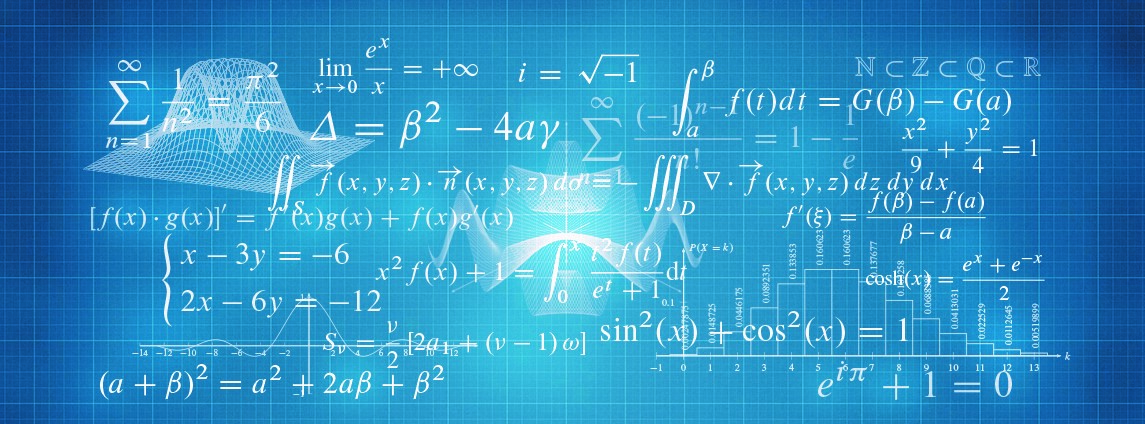
\includegraphics[width=17cm]{Kefalaio}};
\node[anchor=west,xshift=.1\paperwidth,yshift=.14\paperheight,rectangle]
{{\color{white}\fontsize{30}{20}\textbf{\textcolor{black}{\contour{white}{ΚΕΦΑΛΑΙΟ}}}}};
\node[anchor=west,xshift=.09\paperwidth,yshift=.08\paperheight,rectangle] {\fontsize{24}{20} {\color{black}{{\textcolor{black}{\contour{white}{\sc##1}}}}}};
%\fill[fill=black] (12.2,2) rectangle (14.8,4.7);
\node[anchor=west,xshift=.74\paperwidth,yshift=.11\paperheight,rectangle]
{{\color{white}\fontsize{80}{20}\textbf{\textit{\textcolor{white}{\contour{black}{\thechapter}}}}}};
\end{tikzpicture}
};
\end{tikzpicture}
}
\titlespacing*{\chapter}{0pt}{20pt}{30pt}
}
%------------------------------------------------


\usepackage[outline]{contour}
\newcommand{\regularchapter}{%
\titleformat{\chapter}[display]
{\normalfont\huge\bfseries}{\chaptertitlename\ \thechapter}{20pt}{\Huge##1}
\titlespacing*{\chapter}
{0pt}{-20pt}{40pt}
}

\apptocmd{\mainmatter}{\fancychapter}{}{}
\apptocmd{\backmatter}{\regularchapter}{}{}
\apptocmd{\frontmatter}{\regularchapter}{}{}

\titlespacing*{\section}
{0pt}{30pt}{0pt}
\usepackage{booktabs}
\usepackage{hhline}
\DeclareRobustCommand{\perthousand}{%
\ifmmode
\text{\textperthousand}%
\else
\textperthousand
\fi}


\contentsmargin{0cm}
\titlecontents{part}[-1pc]
{\addvspace{10pt}%
\bf\Large ΜΕΡΟΣ\quad }%
{}
{}
{\;\dotfill}%
%------------------------------------------
\titlecontents{chapter}[0pc]
{\addvspace{30pt}%
\begin{tikzpicture}[remember picture, overlay]%
\draw[fill=black,draw=black] (-.3,.5) rectangle (3.7,1.1); %
\pgftext[left,x=0cm,y=0.75cm]{\color{white}\sc\Large\bfseries Κεφάλαιο\ \thecontentslabel};%
\end{tikzpicture}\large\sc}%
{}
{}
{\hspace*{-2.3em}\hfill\normalsize Σελίδα \thecontentspage}%
\titlecontents{section}[2.4pc]
{\addvspace{1pt}}
{\contentslabel[\thecontentslabel]{2pc}}
{}
{\;\dotfill\;\small \thecontentspage}
[]
\titlecontents*{subsection}[4pc]
{\addvspace{-1pt}\small}
{}
{}
{\ --- \small\thecontentspage}
[ \textbullet\ ][]

\makeatletter
\renewcommand{\tableofcontents}{%
\chapter*{%
\vspace*{-20\p@}%
\begin{tikzpicture}[remember picture, overlay]%
\pgftext[right,x=12cm,y=0.2cm]{\Huge\sc\bfseries \contentsname};%
\draw[fill=black,draw=black] (9.5,-.75) rectangle (12.5,1);%
\clip (9.5,-.75) rectangle (15,1);
\pgftext[right,x=12cm,y=0.2cm]{\color{white}\Huge\bfseries \contentsname};%
\end{tikzpicture}}%
\@starttoc{toc}}
\makeatother

\usepackage[contents={},scale=1,opacity=1,color=black,angle=0]{background}

\newcommand\blfootnote[1]{%
\begingroup
\renewcommand\thefootnote{}\footnote{#1}%
\addtocounter{footnote}{-1}%
\endgroup
}
\usepackage{epstopdf}
\epstopdfsetup{update}
\usepackage{textcomp}

\titleformat{\section}
{\normalfont\Large\bf}%
{}{0em}%
{{\color{black}\titlerule[0pt]}\vskip-.2\baselineskip{\parbox[t]{\dimexpr\textwidth-2\fboxsep\relax}{\raggedright\strut\itshape{\LARGE{\thesection~#1}}\strut}}}[\vskip 0\baselineskip{\color{black}\titlerule[1pt]}]
\titlespacing*{\section}{0pt}{0pt}{30pt}

\newcommand{\methodologia}{\begin{center}
{\large \textbf{ΜΕΘΟΔΟΛΟΓΙΑ}}\\\vspace{-2mm}
\begin{tikzpicture}
\shade[left color=white, right color=black,] (-3cm,0) rectangle (0,.2mm);
\shade[left color=black, right color=white,] (0,0) rectangle (3cm,.2mm);   
\end{tikzpicture}
\end{center}}

\newcommand{\orismoi}{\begin{center}
\vspace{-3mm}{\large \textbf{ΟΡΙΣΜΟΙ}}\\\vspace{-2mm}
\begin{tikzpicture}
\shade[left color=white, right color=black,] (-3cm,0) rectangle (0,.2mm);
\shade[left color=black, right color=white,] (0,0) rectangle (3cm,.2mm);   
\end{tikzpicture}
\end{center}}
\newcommand{\thewrhmata}{\begin{center}
{\large \textbf{ΘΕΩΡΗΜΑΤΑ - ΠΟΡΙΣΜΑΤΑ - ΠΡΟΤΑΣΕΙΣ\\ΚΡΙΤΗΡΙΑ - ΙΔΙΟΤΗΤΕΣ}}\\\vspace{-2mm}
\begin{tikzpicture}
\shade[left color=white, right color=black,] (-5cm,0) rectangle (0,.2mm);
\shade[left color=black, right color=white,] (0,0) rectangle (5cm,.2mm);   
\end{tikzpicture}
\end{center}}
\usepackage[labelfont={footnotesize,it,bf},font={footnotesize}]{caption}
\usepackage{systeme,regexpatch}
\makeatletter
% change the definition of \sysdelim not to store `\left` and `\right`
\def\sysdelim#1#2{\def\SYS@delim@left{#1}\def\SYS@delim@right{#2}}
\sysdelim\{. % reinitialize
% patch the internal command to use
% \LEFTRIGHT<left delim><right delim>{<system>}
% instead of \left<left delim<system>\right<right delim>
\regexpatchcmd\SYS@systeme@iii
{\cB.\c{SYS@delim@left}(.*)\c{SYS@delim@right}\cE.}
{\c{SYS@MT@LEFTRIGHT}\cB\{\1\cE\}}
{}{}
\def\SYS@MT@LEFTRIGHT{%
\expandafter\expandafter\expandafter\LEFTRIGHT
\expandafter\SYS@delim@left\SYS@delim@right}
\makeatother
\newcommand{\synt}[2]{{\scriptsize \begin{matrix}
\times#1\\\\ \times#2
\end{matrix}}}
%----------------------------------------
\usepackage{wrapfig}
%-------- ΜΑΘΗΜΑΤΙΚΑ ΕΡΓΑΛΕΙΑ ---------
\usepackage{mathtools}
%----------------------
%-------- ΠΙΝΑΚΕΣ ---------
\usepackage{booktabs}
%----------------------
%----- ΥΠΟΛΟΓΙΣΤΗΣ ----------
%\usepackage{calculator}
%----------------------------
%--------- ΑΝΙΣΩΣΕΙΣ -------
\tikzset{
thickest/.style={line width=1mm},a/.style={decoration={markings,
mark=at position #1 with {\fill[white,draw=black,thin] circle (3pt);}},postaction={decorate}},
k/.style={decoration={markings,
mark=at position #1 with {\fill[black] circle (3pt);}},postaction={decorate}},
}
%--------- ΔΙΑΣΤΗΜΑ ------------
\newcommand{\diasthma}[7]{
\foreach \x in {#3,#4}
\draw (\x,#7+.2) -- (\x,#7-.2);
\node[anchor=north,fill=white] at (#3,#7)[below=1mm] {$ #1 $};
\node[anchor=north,fill=white] at (#4,#7)[below=1mm] {$ #2 $};
\draw [#5=0,#6=1,thickest] (#3,#7)--(#4,#7);
}
%--------- ΑΞΟΝΑΣ ------------------
\newcommand{\axonas}[3]{
\draw[-latex] (#1,#3) -- (#2,#3)node[right]{$x$};
}
%--------- ΚΑΤΩ ΑΚΡΟ ------------------
\newcommand{\Xapeiro}[5]{
\draw (#2,#5+.2) -- (#2,#5-.2);
\node[anchor=north,fill=white] at (#2,#5)[below=1mm] {$ #1 $};
\draw [#4=0,thickest] (#2,#5)--(#3-.3,#5);
}
%--------- ΠΑΝΩ ΑΚΡΟ ------------------
\newcommand{\apeiroX}[5]{
\draw (#2,#5+.2) -- (#2,#5-.2);
\node[anchor=north,fill=white] at (#2,#5)[below=1mm] {$ #1 $};
\draw [#4=0,thickest] (#2,#5)--(#3+.3,#5);
}
%----- ΔΙΑΚΕΚΟΜΜΕΝΕΣ ΓΡΑΜΜΕΣ ------
\newcommand{\oria}[3]{\draw [dashed] (#1,#2)--(#1,#3);}
%--------------------------------------
%----- ΟΡΙΖΟΝΤΙΑ ΛΙΣΤΑ ------
\usepackage{xparse}
\newcounter{answers}
\renewcommand\theanswers{\arabic{answers}}
\ExplSyntaxOn
\NewDocumentCommand{\results}{m}
{
\seq_set_split:Nnn \l_results_a_seq {,}{#1}
\par\nobreak\noindent\setcounter{answers}{0}
\seq_map_inline:Nn \l_results_a_seq
{
\makebox[.18\linewidth][l]{\stepcounter{answers}\theanswers.~##1}\hfill
}
\par
}
\seq_new:N \l_results_a_seq
\ExplSyntaxOff
%----------------------------
%------ ΜΗΚΟΣ ΓΡΑΜΜΗΣ ΚΛΑΣΜΑΤΟΣ ---------
\DeclareRobustCommand{\frac}[3][0pt]{%
{\begingroup\hspace{#1}#2\hspace{#1}\endgroup\over\hspace{#1}#3\hspace{#1}}}
%----------------------------------------
\usepackage{microtype}
\usepackage{float}
\newcommand{\hm}[1]{\textrm{ημ}#1}
\newcommand{\syn}[1]{\textrm{συν}#1}
\newcommand{\ef}[1]{\textrm{εφ}#1}
\newcommand{\syf}[1]{\textrm{σφ}#1}
\usepackage{caption}
%----------- ΓΡΑΦΙΚΕΣ ΠΑΡΑΣΤΑΣΕΙΣ ---------
\pgfkeys{/pgfplots/aks_on/.style={axis lines=center,
xlabel style={at={(current axis.right of origin)},xshift=1.5ex, anchor=center},
ylabel style={at={(current axis.above origin)},yshift=1.5ex, anchor=center}}}
\pgfkeys{/pgfplots/grafikh parastash/.style={black,line width=.4mm,samples=200}}
\pgfkeys{/pgfplots/belh ar/.style={tick label style={font=\scriptsize},axis line style={-latex}}}
%-----------------------------------------
%--------- ΟΡΙΣΜΑ --------------
\newcommand{\Arg}[9]{
\draw[-latex] (#7,#8)-- ++(#1:#2) node[#9=#5]{\footnotesize$#4$};
\draw[fill=black!#6] (#7+0.3+#3,#8) arc (0:#1:0.3+#3) -- (#7,#8);}
%-------------------------------
%---- ΟΡΙΖΟΝΤΙΟ - ΚΑΤΑΚΟΡΥΦΟ - ΠΛΑΓΙΟ ΑΓΚΙΣΤΡΟ ------
\newcommand{\orag}[3]{\node at (#1)
{$ \overcbrace{\rule{#2mm}{0mm}}^{{\scriptsize #3}} $};}

\newcommand{\kag}[3]{\node at (#1)
{$ \undercbrace{\rule{#2mm}{0mm}}_{{\scriptsize #3}} $};}

\newcommand{\Pag}[4]{\node[rotate=#1] at (#2)
{$ \overcbrace{\rule{#3mm}{0mm}}^{{\rotatebox{-#1}{\scriptsize$#4$}}}$};}
%-----------------------------------------
\tikzstyle{pl}=[line width=0.3mm]
\tikzstyle{plm}=[line width=0.4mm]
%------- ΣΤΥΛ ΠΑΡΑΔΕΙΓΜΑΤΟΣ -------
\newcounter{paradeigma}[section]
\renewcommand{\theparadeigma}{\bf\arabic{paradeigma}\;:\;}   
\newcommand{\Paradeigma}[1]{\refstepcounter{paradeigma}\textcolor{black}{\textbf{ΠΑΡΑΔΕΙΓΜΑ\hspace{2mm}\theparadeigma\hspace{1mm}}} \MakeUppercase{\textbf{#1}}\\}{}
%-----------------------------------

%------- ΣΤΥΛ ΛΥΣΗΣ ------------------
\newcommand{\lysh}{{\textbf{ΛΥΣΗ}}}
%------------------------------------

%------ ΛΥΜΕΝΑ ΠΑΡΑΔΕΙΓΜΑΤΑ ΤΙΤΛΟΣ ---------
\newcommand{\Lymena}{\begin{center}
\begin{tikzpicture}
\fill[black] (-7cm,-.6cm) rectangle (6.5cm,.6cm);
\node at (-.25cm,0) {\Large \textcolor{white}{\textbf{ΛΥΜΕΝΑ ΠΑΡΑΔΕΙΓΜΑΤΑ}}};  
\end{tikzpicture}
\end{center}}
%--------------------------------------

%--------- ΑΛΥΤΕΣ ΑΣΚΗΣΕΙΣ ΤΙΤΛΟΣ ----------
\newcommand{\Alyta}{\begin{center}
\begin{tikzpicture}
\fill[black] (-7cm,-.6cm) rectangle (6.5cm,.6cm);
\node at (-.25cm,0) {\Large \textcolor{white}{\textbf{ΑΣΚΗΣΕΙΣ - ΠΡΟΒΛΗΜΑΤΑ}}};  
\end{tikzpicture}
\end{center}}
%--------------------------------------------
%---------- ΜΕΘΟΔΟΣ --------------
\newcounter{Methodos}[section]
\renewcommand{\theMethodos}{\arabic{Methodos}} 
\newenvironment{Methodos}[1][]{%
\refstepcounter{Methodos}
\begin{mdframed}[%
frametitle={\vspace{-1.5mm}\begin{center}
{ΜΕΘΟΔΟΣ \;\;\theMethodos\;:\quad\ \MakeUppercase{#1}}
\end{center}\vspace{.5mm}},
skipabove=\baselineskip plus 0pt minus 1pt,
skipbelow=\baselineskip plus 2pt minus 1pt,
linewidth=0pt,
frametitlerule=true,
frametitlebackgroundcolor=black!50,
linecolor=black,
outerlinewidth=0pt,
rightline=false,
bottomline=false,
topline=false,
frametitlerulewidth=.3pt,
innertopmargin=\baselineskip,
innerbottommargin=4mm,
innerrightmargin=20pt,
innerleftmargin=20pt,
backgroundcolor=black!10,
frametitleaboveskip=7pt
]%
}{%
\end{mdframed}}
%------------------------------------------
%---------- ΛΙΣΤΕΣ ----------------------
\newlist{bhma}{enumerate}{3}
\setlist[bhma]{label=\bf\textit{\arabic*\textsuperscript{o}\;Βήμα :},leftmargin=0cm,itemindent=1.5cm,ref=\bf{\arabic*\textsuperscript{o}\;Βήμα}}
\newlist{rlist}{enumerate}{3}
\setlist[rlist]{itemsep=0mm,label=\roman*.}
\newlist{brlist}{enumerate}{3}
\setlist[brlist]{itemsep=0mm,label=\bf\roman*.}
\newlist{tropos}{enumerate}{3}
\setlist[tropos]{label=\bf\textit{\arabic*\textsuperscript{oς}\;Τρόπος :},leftmargin=0cm,itemindent=2.3cm,ref=\bf{\arabic*\textsuperscript{oς}\;Τρόπος}}
% Αν μπει το bhma μεσα σε tropo τότε
%\begin{bhma}[leftmargin=.7cm]
%----------- ΓΡΑΦΙΚΕΣ ΠΑΡΑΣΤΑΣΕΙΣ ---------
\pgfkeys{/pgfplots/aks_on/.style={axis lines=center,
xlabel style={at={(current axis.right of origin)},xshift=1.5ex, anchor=center},
ylabel style={at={(current axis.above origin)},yshift=1.5ex, anchor=center}}}
\pgfkeys{/pgfplots/grafikh parastash/.style={black,line width=.4mm,samples=200}}
\pgfkeys{/pgfplots/belh ar/.style={tick label style={font=\scriptsize},axis line style={-latex}}}
%-----------------------------------------
\tkzSetUpPoint[size=7,fill=white]
\newcommand{\tss}[1]{\textsuperscript{#1}}
\newcommand{\tssL}[1]{\MakeLowercase{\textsuperscript{#1}}}
%------------------------------------------
\usepackage{extarrows}
\newcommand{\eq}[1]{\xlongequal{#1}}
\newcommand{\eqq}[2]{\xlongequal[#2]{#1}}
\DeclareMathOperator*{\Eq}{=}
%------------------------------------------






\begin{document}
\title{\MakeUppercase{ΣΧΟΛΙΚΟ ΤΥΠΟΛΟΓΙΟ}}
\pagestyle{empty}
\frontmatter
\begin{titlepage}
\newgeometry{left=2.5cm,top=2.5cm} %defines the geometry for the titlepage
\pagecolor{white}
\begin{center}
{\large Σπύρος Φρόνιμος\\Μαθηματικός}
\end{center}
\noindent
\par
\noindent
\mbox{}\\\\
\begin{center}
\textbf{\fontsize{25}{40}\selectfont{ΜΑΘΗΜΑΤΙΚΑ}}\par\mbox{}\\\vspace{-3mm}
\textbf{\fontsize{25}{40}\selectfont{Γ΄ ΓΥΜΝΑΣΙΟΥ}}\par\mbox{}\\
\vspace{-4mm}
\rule{12cm}{0.1mm}\\
\vspace{3mm}
{\fontsize{15}{15}\MakeUppercase{τύποι ορισμοί θεωρήματα και}}\\
\vspace{.7mm}
{\fontsize{15}{15}\MakeUppercase{βασική μεθοδολογία των μαθηματικων}}\\
\vspace{.7mm}
{\fontsize{15}{15}\MakeUppercase{της γ΄ γυμνασιου}}\\
\rule{12cm}{0.1mm}\\
\end{center}
\vspace{3cm}
\begin{flushright}
\begin{itemize}
\item 100 Ορισμοί
\item 250 Θεωρήματα
\item 400 Μέθοδοι για λύση ασκήσεων
\item 200 Λυμένα παραδείγματα
\item 500 Άλυτες ασκήσεις και προβλήματα
\item 200 Επαναληπτικά θέματα
\item Απαντήσεις ασκήσεων
\end{itemize}
\end{flushright}

\vfill
\noindent
\color{black}
\begin{center}
{\large{ΕΚΔΟΣΕΙΣ \_\_\_\_\_}\\
\large{ΚΕΡΚΥΡΑ 2015}}
\vskip\baselineskip
\end{center}
\hbox{ % Horizontal box
\hspace*{0.2\textwidth} % Whitespace to the left of the title page
\rule{1pt}{\textheight} % Vertical line
\hspace*{0.05\textwidth} % Whitespace between the vertical line and title page text
\parbox[b]{0.75\textwidth}{ % Paragraph box which restricts text to less than the width of the page

{\textbf{ΜΑΘΗΜΑΤΙΚΑ}\\\textbf{Γ΄ Γυμνασίου}\\\\\noindent \textbf{Σπύρος Φρόνιμος - Μαθηματικός}\\e-mail : spyrosfronimos@gmail.com\\[0.5\baselineskip]
Σελίδες : ...\\
ΙΣΒΝ : ...\\
Εκδόσεις : ...\\
\textcopyright Copyright 2015}\\[2\baselineskip] % Title
{Φιλολογική Επιμέλεια :\\\textbf{Μαρία Πρεντουλή}}
{- e-mail : predouli@yahoo.com}\\[0.5\baselineskip]
{Επιστημονική Επιμέλεια :}{\textbf{Σπύρος Φρόνιμος}}\\[0.5\baselineskip]
{Εξώφυλλο : \\\textbf{Δημήτρης Πρεντουλής}}\\[1\baselineskip] % Tagline or further description
% Author name

\vspace{.4\textheight} % Whitespace between the title block and the publisher
{Πνευματικά Δικαιώματα : ...}\\[\baselineskip]}}
\vspace*{2\baselineskip}
\newpage
\mbox{}\\\\\\\\\\\\
\hspace*{0.75\textwidth}
\textit{{\large Στη γυναίκα μου.}}
\newpage
\mbox{}
\newpage
\mbox{}
{\LARGE \textbf{Πρόλογος}}\\\\\\\\

Το βιβλίο περιέχει συγκεντρωμένη όλη τη θεωρία των μαθηματικών όλων των τάξεων του γυμνασίου και του λυκείου γραμμένη αναλυτικά και κατανοητά.\\\\
Ειδικότερα ο αναγνώστης θα βρει\\
\vspace{-.4cm}
\begin{itemize}
\item Ορισμούς
\item Θεωρήματα
\item Τυπολόγιο
\item Μεθοδολογία
\end{itemize}
Σκοπό έχει να αποτελέσει ένα χρήσιμο βοήθημα για μικρούς ή μεγάλους μαθητές όπου μπορούν να έχουν όλη τη θεωρία της χρονιάς τους συγκεντρωμένη, χρήσιμη για επανάληψη και διαγωνίσματα, αλλά και να μπορούν εύκολα να καλύψουν τυχόν κενά από προηγούμενες τάξεις.\\\\\\
Θέλω να ευχαριστήσω όλους όσους βοήθησαν.
\newpage
\end{titlepage}
\restoregeometry % restores the geometry
\tableofcontents
\mainmatter
\part{ΑΛΓΕΒΡΑ}
\pagestyle{fancy}
\chapter{Πραγματικοί Αριθμοί}
\section{Πράξεις μεταξύ πραγματικών αριθμών}
\orismoi
\Orismos{Σύνολα αριθμών}
Τα βασικά σύνολα αριθμών που έχουμε μελετήσει συνοψίζονται στην παρακάτω λίστα.
\begin{enumerate}[itemsep=0mm,label=\bf\arabic*.]
\item \textbf{Φυσικοί Αριθμοί} : Το σύνολο των αριθμών από το 0 εως το άπειρο όπου κάθε αριθμός έχει διαφορά μιας μονάδας από τον προηγούμενο.
\item \textbf{Ακέραιοι Αριθμοί}: Το σύνολο των φυσικών αριθμών μαζί με τους αντίθετους τους.
\item \textbf{Ρητοί Αριθμοί}: Όλοι οι αριθμοί που μπορούν να γραφτούν με τη μορφή κλάσματος με ακέραιους όρους.
\item \textbf{Άρρητοι Αριθμοί}: Κάθε αριθμός ο οποίος δεν είναι ρητός. Κατά κύριο λόγο, άρρητοι αριθμοί είναι οι ρίζες που δεν έχουν ρητό αποτέλεσμα, ο αριθμός $ \pi $ κ.τ.λ.
\item \textbf{Πραγματικοί Αριθμοί} : Οι ρητοί μαζί με το σύνολο των άρρητων μας δίνουν τους πραγματικούς αριθμούς, όλους τους αριθμούς που γνωρίζουμε.
\end{enumerate}
\Orismos{Αντίθετοι - Αντίστροφοι αριθμοι}
Για τις πράξεις της πρόσθεσης και του πολλαπλασιασμού ορίζουμε στο σύνολο των πραγματικών αριθμών τα εξής :
\begin{enumerate}[itemsep=0mm,label=\bf\arabic*.]
\item \textbf{Αντίθετοι αριθμοί}\\
Αντίθετοι ονομάζονται οι αριθμοί οι οποίοι έχουν άθροισμα μηδέν. Οι αντίθετοι αριθμοί έχουν ίσες απόλυτες τιμές και αντίθετα πρόσημα.
\[ a+(-a)=0 \]
\item \textbf{Αντίστροφοι αριθμοί}\\
Αντίστροφοι ονομάζονται δύο πραγματικοί αριθμοί οι οποίοι έχουν γινόμενο ίσο με τη μονάδα. \[ a\cdot \frac{1}{a}=1 \]
\end{enumerate}
\Orismos{Πράξεισ αριθμών}
Στον παρακάτω πίνακα φαίνονται τα ονόματα των αριθμών που αποτελούν μια πράξη, τα ονόματα των αποτελεσμάτων και ο συμβολισμός κάθε πράξης.
\begin{center}
\begin{longtable}{cccc}
\hline \rule[-2ex]{0pt}{5.5ex} \textbf{Πράξη} & \textbf{Όροι} & \textbf{Αποτέλεσμα} & \textbf{Συμβολισμός} \\ 
\hhline{====} \rule[-2ex]{0pt}{5.5ex} \textbf{Πρόσθεση} & Προσθετέοι & Άθροισμα & $ a+\beta $ \\ 
\rule[-2ex]{0pt}{5.5ex} \textbf{Αφαίρεση} & Μειωτέος - Αφαιρετέος & Διαφορά & $ a-\beta $ \\ 
\rule[-2ex]{0pt}{5.5ex} \textbf{Πολλαπλασιασμός} & Παράγοντες & Γινόμενο & $ a\cdot\beta $ \\ 
\rule[-2ex]{0pt}{5.5ex} \textbf{Διαίρεση} & Διαιρετέος - Διαιρέτης & Πηλίκο & $ a:\beta $ \\ 
\hline\end{longtable}
\end{center}
\vspace{-5mm}
Η αφαίρεση $ a-\beta $ και η διαίρεση $ a:\beta $ δύο αρθμών $ a,\beta\in\mathbb{R} $ είναι οι πράξεις που προκύπτουν από την πρόσθεση και τον πολλαπλασιασμό αντίστοιχα και μπορούν να γραφτούν με τη βοήθεια τους.
\[ a-\beta=a+(-\beta)\;\;,\;\;a:\beta=\frac{a}{\beta}=a\cdot\frac{1}{\beta} \]
\Orismos{Απόλυτη Τιμή Πραγματικού Αριθμού}
Απόλυτη τιμή ενός πραγματικού αριθμού  ορίζεται να είναι η απόσταση της εικόνας του αριθμού αυτού απο το 0 και συμβολίζεται με $ |a| $.
\begin{center}
\begin{longtable}{c >{\centering\arraybackslash}m{6cm}}
$ |a|=\LEFTRIGHT\{.{\begin{aligned}
a & \;,\;a\geq0\\
-a & \;,\;a<0
\end{aligned}} $  & \begin{tikzpicture}
\draw[-latex] (-1,0) -- coordinate (x axis mid) (4.4,0) node[right,fill=white] {{\footnotesize $ x $}};
\foreach \x in {-1,0,...,4}
\draw (\x,.5mm) -- (\x,-.5mm) node[anchor=north,fill=white] {{\scriptsize \x}};
\draw[line width=.7mm] (0,0) -- (3,0);
\tkzText(1.5,.34){$ \overcbrace{\rule{27mm}{0mm}}^{{\scriptsize |3|=3}} $}
\tkzDefPoint(3,0){A}
\tkzDrawPoint[size=7,fill=white](A)
\tkzLabelPoint[above right,xshift=-2mm](A){{\scriptsize $A(3)$}}
\end{tikzpicture}
\end{longtable} 
\end{center}
\begin{itemize}[itemsep=0mm]
\item Η απόλυτη τιμή ενός θετικού αριθμού $ a $ είναι ίση με τον ίδιο τον αριθμό.
\item Η απόλυτη τιμή ενός αρνητικού αριθμού $ a $ είναι ίση με τον αντίθετο του αριθμού $ a $.
\end{itemize}
Η απόλυτη τιμή ενός πραγματικού αριθμού είναι θετικός αριθμός αφού εξ' ορισμού παριστάνει απόσταση, που σαν μέγεθος παιρνει μόνο θετικές τιμές.
\thewrhmata
\Thewrhma{Ιδιότητεσ των Πράξεων}
Στον παρακάτω πίνακα βλέπουμε τις βασικές ιδιότητες της πρόσθεσης και του πολλαπλασιασμού στο σύνολο των πραγματικών αριθμών.
\begin{center}
\begin{longtable}{ccc}
	\hline \rule[-2ex]{0pt}{5.5ex} \textbf{Ιδιότητα} & \textbf{Πρόσθεση} & \textbf{Πολλαπλασιασμός} \\ 
	\hhline{===} \rule[-2ex]{0pt}{5.5ex} \textbf{Αντιμεταθετική} & $ a+\beta=\beta+a $ & $ a\cdot\beta=\beta\cdot a $ \\
	\rule[-2ex]{0pt}{5ex} \textbf{Προσεταιριστική} & $ a+\left( \beta+\gamma\right) =\left( a+\beta\right) +\gamma $ & $ a\cdot\left( \beta\cdot\gamma\right) =\left( a\cdot\beta\right)\cdot\gamma $\\
	\rule[-2ex]{0pt}{5ex} \textbf{Ουδέτερο στοιχείο} & $ a+0=a $ & $ a\cdot1= a $\\
	\rule[-2ex]{0pt}{5ex} \textbf{Αντίθετοι / Αντίστροφοι} & $ a+(-a)=0 $ & $ a\cdot\frac{1}{a}= 1 $\\
	\rule[-2ex]{0pt}{5ex} \textbf{Επιμεριστική} & \multicolumn{2}{c}{$ a\cdot\left( \beta\pm\gamma\right)=a\cdot\beta\pm a\cdot\gamma  $}\\
	\hline
\end{longtable}
\end{center}
\vspace{-7mm}
Ισχύουν επίσης :
\begin{itemize}[itemsep=0mm]
\item Για κάθε πραγματικό αριθμό $ a $ ισχύει $ a\cdot0=0 $
\item Δύο αριθμοί που έχουν άθροισμα 0 λέγονται \textbf{αντίθετοι}.
\item Το 0 λέγεται \textbf{ουδέτερο στοιχείο της πρόσθεσης}.
\item Δύο αριθμοί που έχουν γινόμενο 1 λέγονται \textbf{αντίστροφοι}.
\item Το 1 λέγεται \textbf{ουδέτερο στοιχείο του πολλαπλασιασμού}.
\item Το 0 δεν έχει αντίστροφο.
\end{itemize}
\Thewrhma{Γινόμενο - Πηλίκο πραγματικων αριθμών}
Για οποιουσδήποτε δύο πραγματικούς $ a,\beta\in\mathbb{R} $ ισχύουν οι παρακάτω προτάσεις :
\begin{itemize}[itemsep=0mm]
\item Το γινόμενο και το πηλίκο δύο ομόσημων πραγματικών αριθμών $ a,\beta $ είναι θετικό.
\item Το γινόμενο και το πηλίκο δύο ετερόσημων πραγματικών αριθμών $ a,\beta $ είναι αρνητικό.
\end{itemize}
\begin{gather*}
a,\beta\textrm{ ομόσημοι }\Rightarrow a\cdot\beta>0\textrm{ και }\dfrac{a}{\beta}>0\\
a,\beta\textrm{ ετερόσημοι }\Rightarrow a\cdot\beta<0\textrm{ και }\dfrac{a}{\beta}<0
\end{gather*}
\section{Δυνάμεις}
\orismoi
\Orismos{Δύναμη πραγματικου αριθμου}
Δύναμη ενός πραγματικού αριθμού $ a $ ονομάζεται το γινόμενο $ \nu $ ίσων παραγόντων του αριθμού αυτού. Συμβολίζεται με $ a^\nu $ όπου ο φυσικός αριθμός $ \nu $ είναι το πλήθος των ίσων παραγόντων. 
\[ \undercbrace{a\cdot a\cdot\ldots a}_{\nu\textrm{ παράγοντες }}=a^\nu \]
\begin{itemize}[itemsep=0mm]
\item Ο αριθμός $ a $ ονομάζεται \textbf{βάση} και ο αριθμός $ \nu $ \textbf{εκθέτης} της δύναμης.
\item Η δύναμη $ a^2 $ ονομάζεται και $ \mathbold{a} $ \textbf{στο τετράγωνο}.
\item Η δύναμη $ a^3 $ ονομάζεται και  {\boldmath $ a $}  \textbf{στον κύβο}.
\end{itemize}
Επίσης για κάθε δύναμη με βάση έναν πραγματικό αριθμό $ a $ ορίζουμε
\begin{multicols}{3}
\begin{itemize}
\item $ a^1=a $
\item $ a^0=1\ ,\ a\neq 0 $
\item $ a^{-\nu}=\frac{1}{a^\nu}\ ,\ a\neq 0 $
\end{itemize}
\end{multicols}
\thewrhmata
\Thewrhma{Ιδιότητεσ Δυνάμεων}
Για κάθε δυναμη με βάση οποιουσδήποτε πραγματικούς αριθμούς $ a,\beta $ και φυσικούς εκθέτες $ \nu,\mu $ ισχύουν οι παρακάτω ιδιότητες :
\begin{center}
\begin{longtable}{ccc}
\hline \rule[-2ex]{0pt}{5.5ex} & \textbf{Ιδιότητα} & \textbf{Συνθήκη} \\
\hhline{===}\rule[-2ex]{0pt}{5.5ex} \textbf{1} & Γινόμενο δυνάμεων με κοινή βάση & $ a^\nu\cdot a^\mu=a^{\nu+\mu} $ \\
\rule[-2ex]{0pt}{5.5ex} \textbf{2} & Πηλίκο δυνάμεων με κοινή βάση & $ a^\nu: a^\mu=a^{\nu-\mu} $\\
\rule[-2ex]{0pt}{5.5ex} \textbf{3} & Γινόμενο δυνάμεων με κοινό εκθέτη & $ \left(a\cdot\beta\right)^\nu=a^\nu\cdot\beta^\nu $ \\
\rule[-2ex]{0pt}{5.5ex} \textbf{4} & Πηλίκο δυνάμεων με κοινό εκθέτη & $ \left(\dfrac{a}{\beta}\right)^\nu=\dfrac{a^\nu}{\beta^\nu}\;\;,\;\;\beta\neq0 $ \\
\rule[-2ex]{0pt}{5.5ex} \textbf{5} & Δύναμη υψωμένη σε δύναμη & $ \left( a^\nu\right)^\mu=a^{\nu\cdot\mu} $ \\
\rule[-2ex]{0pt}{5.5ex} \textbf{6} & Κλάσμα με αρνητικό εκθέτη & $ \left( \dfrac{a}{\beta}\right)^{-\nu}=\left(\dfrac{\beta}{a}\right)^\nu\;\;,\;\;a,\beta\neq0 $ \\
&&\\
\hline
\end{longtable}
\end{center}
\vspace{-5mm}
Οι ιδιότητες 1 και 3 επεκτείνονται και για το γινόμενο περισσότερων των δύο παραγόντων. Για οπουσδήποτε πραγματικούς αριθμούς $ a, a_1, a_2,\ldots,a_\kappa $ και φυσικούς εκθέτες $ \nu, \nu_1,\nu_2,\ldots,\nu_\kappa $ θα ισχύει :
\begin{gather*}
a^{\nu_1}\cdot a^{\nu_2}\cdot\ldots\cdot a^{\nu_\kappa}=a^{\nu_1+\nu_2+\ldots+\nu_\kappa}\\
\left( a_1\cdot a_2\cdot\ldots\cdot a_\kappa\right)^\nu=a_1^\nu\cdot a_2^\nu\cdot\ldots\cdot a_\kappa^\nu
\end{gather*}
\section{Τετραγωνική ρίζα}
\orismoi
\Orismos{Τετραγωνική Ρίζα}
Τετραγωνική ρίζα ενός θετικού αριθμού $ x $ ονομάζεται ο \textbf{θετικός} αριθμός $ a $ που αν υψωθεί στο τετράγωνο δίνει τον αριθμό $ x $ και συμβολίζεται με $ \sqrt{x} $.
\[ \sqrt{x}=a\;\;,\;\;\textrm{ όπου }x\geq0\textrm{ και }a\geq0 \]
\begin{itemize}[itemsep=0mm]
\item Δεν ορίζεται ρίζα αρνητικού αριθμού.
\item Ο θετικός αριθμός $ x $ ονομάζεται \textbf{υπόριζο}.
\end{itemize}
\thewrhmata
\Thewrhma{Ιδιότητεσ Ριζών}
Για οποιουσδήποτε πραγματικούς αριθμούς $ x,y $ ισχύουν οι παρακάτω ιδιότητες που αφορούν την τετραγωνική τους ρίζα.
\begin{center}
\begin{longtable}{ccc}
\hline \rule[-2ex]{0pt}{5.5ex} & \textbf{Ιδιότητα} & \textbf{Συνθήκη} \\
\hhline{===}\rule[-2ex]{0pt}{5.5ex} \textbf{1} & Τετράγωνο ρίζας & $ \left(\sqrt{x}\;\right)^2=x\;\;,\;\; x\geq0  $ \\
\rule[-2ex]{0pt}{5.5ex} \textbf{2} & Ρίζα τετραγώνου & $ \sqrt{x^2}=|x|\;\;,\;\; x\;\textrm{ πραγματικός} $\\
\rule[-2ex]{0pt}{5.5ex} \textbf{3} & Ρίζα γινομένου & $ \sqrt{x\cdot y}=\!\sqrt{x}\cdot\!\sqrt{y}\;\;,\;\; x,y\geq0 $ \\
\rule[-2ex]{0pt}{6.5ex}\textbf{4} & Ρίζα πηλίκου & $ \SQRT{\dfrac{x}{y}}=\dfrac{\sqrt{x}}{\sqrt{y}}\;\;,\;\;x\geq0\textrm{ και }y>0 $ \vspace{1mm}\\
\hline
\end{longtable}
\end{center}
Η ιδιότητα 3 ισχύει και για το γινόμενο περισσότερων των δύο παραγόντων. Έτσι αν $ x_1,x_2,\ldots,x_\nu $ είναι $ \nu $ σε πλήθος θετικοί πραγματικοί αριθμοί τότε θα ισχύει : \[ \sqrt{x_1\cdot x_2\cdot\ldots\cdot x_\nu}=\!\sqrt{x_1}\cdot\!\sqrt{x_2}\cdot\ldots\cdot\!\sqrt{x_\nu} \] όπου $ x_1,x_2,\ldots x_\nu\geq0 $ και $ \nu\;\textrm{ φυσικός} $.
\Lymena
\begin{Methodos}[Πράξεισ μεταξύ αριθμών]
Σε αριθμητικές παραστάσεις όπου καλούμαστε να κάνουμε πράξεις μεταξύ πραγματικών αριθμών ακολουθούμε τα παρακάτω βήματα για κάθε πράξη
\begin{enumerate}[leftmargin=.5cm,label=\bf\arabic*.]
\item \textbf{Πρόσθεση}
\begin{brlist}[leftmargin=.5cm]
\item Για να προσθέσουμε δύο ομόσημους αριθμούς, προσθέτουμε τις απόλυτες τιμές τους και γράφουμε μπροστά από το αποτέλεσμα το κοινό τους πρόσημο.
\item Για να προσθέσουμε δύο ετερόσημους αριθμούς, αφαιρούμε τις απόλυτες τιμές τους και γράφουμε μπροστά από το αποτέλεσμα το πρόσημο του αριθμού με τη μεγαλύτερη απόλυτη τιμή.
\end{brlist}
\item \textbf{Πολλαπλασιασμός}
\begin{brlist}[leftmargin=.5cm]
\item Για να πολλαπλασιάσουμε δύο ομόσημους αριθμούς, πολλαπλασιάζουμε τις απόλυτες τιμές τους και γράφουμε μπροστά από το αποτέλεσμα το πρόσημο $ + $.
\item Για να πολλαπλασιάσουμε δύο ετερόσημους αριθμούς, πολλαπλασιάζουμε τις απόλυτες τιμές τους και γράφουμε μπροστά από το αποτέλεσμα το πρόσημο $ - $.
\end{brlist}
\end{enumerate}
\end{Methodos}
\Paradeigma{Πράξεισ μεταξύ αριθμών}
\textbf{Να υπολογιστούν οι τιμές των παρακάτω αθροισμάτων και γινομένων}
\begin{multicols}{4}
{\boldmath\begin{rlist}[label=\bf\roman{*.}]
\item $ 17+23 $
\item $ 32-47 $
\item $ 28-15 $
\item $ -54-27 $
\item $ 8\cdot9 $
\item $ (-14)\cdot15 $
\item $ 25\cdot(-8) $
\item $ (-32)\cdot(-100) $
\end{rlist}}
\end{multicols}
\noindent
\lysh\\
Σε κάθε πράξη απο τις παραπάνω εξετάζουμε αν οι αριθμοί είναι ομόσημοι ή ετερόσημοι.
\begin{rlist}
\item Οι αριθμοί της παράστασης είναι ομόσημοι οπότε προσθέτουμε τις απόλυτες τιμές τους. Το αποτέλεσμα θα έχει το ίδιο πρόσημο.
\[ 17+23=+(17+23)=+40=40 \]
\item Στην παράσταση αυτή θα αφαιρέσουμε τις απόλυτες τιμές των αριθμών αφού είναι ετερόσημοι. Το αποτέλεσμα θα έχει το πρόσημο του αριθμού με τη μεγαλύτερη απόλυτη τιμή.
\[ 32-47=-(47-32)=-15 \]
Συνεχίζουμε και στα επόμενα παραδείγματα με τον ίδιο τρόπο.
\item $ 28-15=+(28-15)=+13=13 $
\item $ -54-27=-(54+27)=-81 $
\item Οι παράγοντες του γινομένου είναι ομόσημοι. Επομένως το αποτέλεσμα θα είναι θετικο.
\[ 8\cdot9=+72=72 \]
\item Το γινόμενο αυτό περιέχει ετερόσημους παράγοντες. Το αποτέλεσμα του γινομένου θα είναι αρνητικό.
\[ (-14)\cdot15=-14\cdot15=-210 \]
Ομοίως και στα επόμενα παραδείγματα θα έχουμε
\item $ 25\cdot(-8)=-25\cdot8=-200 $
\item $ (-32)\cdot(-100)=+32\cdot100=3200 $
\end{rlist}
\begin{Methodos}[Αριθμητικέσ παραστάσεισ]
Σε σύνθετες αριθμητικές παραστάσεις, οι οποίες περιέχουν πολλές πράξεις, ακολουθούμε τη σειρά των πράξεων που γνωρίζουμε από την Α' Γυμνασίου δηλαδή
\begin{enumerate}[itemsep=0mm]
\item Πολλαπλασιασμοί - Διαιρέσεις
\item Προσθέσεις - Αφαιρέσεις
\end{enumerate}
Οι πράξεις εκτελούνται με τη σειρά αυτή πρώτα μέσα σε παρενθέσεις, αν υπάρχουν και ύστερα έξω απ' αυτές. Μπορούν οι πολλπλασιασμοί και διαιρέσεις μεταξύ προσήμων και μεταξύ αριθμών να γίνουν σε ξεχωριστά βήματα προκειμένου να αποφύγουμε τα λάθη. Αν υπάρχει εμπειρία μπορούμε να βγάλουμε και κατευθείαν το αποτέλεσμα.
\end{Methodos}
\Paradeigma{Αριθμητική παράσταση}
\textbf{Να βρεθεί η τιμή της παρακάτω αλγεβρικής παράστασης.}
{\boldmath\[ -2\cdot5+4\cdot\left(-\frac{3}{5} \right)-\frac{35}{4}:\left(-\frac{15}{2}\right)   \]}
\lysh\\
Ακολουθώντας τα βήματα που μας υποδεικνύει η μέθοδος θα έχουμε
\begin{align*}
-2\cdot5+4\cdot\left(-\frac{3}{5} \right)-\frac{35}{4}:\left(-\frac{15}{2}\right)&\eq{\textrm{Πρόσημα}}-2\cdot5-4\cdot\frac{3}{5} +\frac{35}{4}:\frac{15}{2}\\
\textrm{Πολλ/μοι - Διαιρέσεις} \qquad&=-10-\frac{12}{5} +\frac{35}{4}\cdot\frac{2}{15}=-10-\frac{12}{5} +\frac{7}{6}\\
\textrm{Προσθ.-Αφαιρ.} \qquad&=-\frac{300}{30}-\frac{72}{30} +\frac{35}{30}=\frac{337}{30}
\end{align*}
\begin{Methodos}[Υπολογισμόσ παραστασησ με αγνωστο αριθμο]
Εαν μια αριθμητική παράσταση περιέχει έναν άγνωστο αριθμό ή αγνωστη παράσταση, των οποίων όμως η τιμή δίνεται γνωστή από την εκφώνση της άσκησης, τότε προκειμένου να υπολογίσουμε την τιμή της παράστασης :
\begin{bhma}
\item \textbf{Αντικατάσταση}\\
Αντικαθιστούμε τον άγνωστο αριθμό με την τιμή του. Στην περίπτωση άγνωστης παράστασης με πολλούς άγνωστους αριθμούς, αντικαθιστούμε ολόκληρη την παράσταση αυτή με την τιμή που μας δίνεται χωρίς να είναι απαραίτητο να γνωρίζουμε την τιμή κάθε αγνώστου ξεχωριστά.
\item \textbf{Πράξεις}\\
Στη συνέχεια εκτελούμε τις πράξεις σύμφωνα με τις οδηγίες της \textbf{Μεθόδου 1} για πραγματικούς αριθμούς ώστε να υπολογίσουμε την τιμή της παράστασης.
\end{bhma}
\end{Methodos}
\Paradeigma{Αριμητική παράσταση με άγνωστο}
{Να υπολογιστεί η αριθμητική τιμή των παρακάτω παραστάσεων}
{\boldmath
\begin{brlist}
\item $ 3x-4+2y-8-4y+x-5 $ \textbf{για} $ x=-2 $ \textbf{και} $ y=3 $
\item $ 2-7y-3-3x+1-x+3y+9 $ \textbf{όταν} $ x+y=4 $
\end{brlist}}
\noindent
\lysh\\
\begin{rlist}
\vspace{-5mm}
\item Στην 1\tss{η} παράσταση γνωρίζουμε την τιμή κάθε μεταβλητής ξεχωριστά. Μπορούμε λοιπόν να αντικαταστήσουμε τις μεταβλητές με τους αριθμούς και να υπολογίσουμε την τιμή. Πριν απ' αυτό θα χρειαστεί να γίνει αναγωγή ομοίων όρων.
\[ 3x-4+2y-8-4y+x-5=4x-2y-17 \]
Με αντικατάσταση θα έχουμε όπου $ x=-2 $ και $ y=3 $
\[ 4x-2y-17=4\cdot(-2)-2\cdot3-17=-8-6-17=-31 \]
\item Στην παράσταση αυτή θα χρειαστεί να απλοποιήσουμε τη μορφή της κάνοντας αναγωγή ομοίων όρων και να εμφανίσουμε την παράσταση $ x+y $ μιας και δεν γνωρίζουμε την τιμή κάθε μεταβλητής ξεχωριστά.
\[ 2-7y-3-3x+1-x+3y+9=-4x-4y+9\eq{\textrm{Επιμ. Ιδ.}}-4(x+y)+9 \]
Αντικαθιστώντας όπου $ x+y=4 $ θα έχουμε
\[ -4(x+y)+9=-4\cdot4+9=-16+9=-7 \]
\end{rlist}
\begin{Methodos}[Υπολογισμόσ αριθμητικών παραστάσεων]
Για τον υπολογισμό αριθμητικών παραστάσεων οι οποίες περιέχουν και δυνάμεις πραγματικών αριθμών, ακολουθούμε τα βήματα που μας υποδεικνύει ο \textbf{Ορισμός 1} για τη σειρά των πράξεων δηλαδή
\begin{bhma}
\item \textbf{Υπολογισμός δυνάμεων}\\
Ξεκινώντας από τις πράξεις που βρίσκονται μέσα σε παρενθέσεις, υπολογίζουμε τις δυνάμεις, κάνοντας χρήση αν χρειαστεί των ιδιοτήτων του \textbf{Θεωρήματος 1}.
\item \textbf{Πολλαπλασιασμοί - Διαιρέσεις}\\
Στη συνέχεια εκτελούμε τους πολλαπλασιασμούς και τις διαιρέσεις τις αριθμητικής παράστασης.
\item \textbf{Προσθέσεις - Αφαιρέσεις}\\
Τέλος, εκτελούμε τις προσθέσεις και τις αφαιρέσεις της παράστασης.
\end{bhma}
Οι πράξεις αυτές επαναλαμβάνονται με την ίδια σειρά και έξω από τις παρενθέσεις, οποτε και προκύπτει το αποτέλεσμα της αριθμητικής παράστασης.
\end{Methodos}
\Paradeigma{Υπολογισμόσ παραστάσεων}
\textbf{Να υπολογιστεί η τιμή της παρακάτω αριθμητικής παράστασης.}
{\boldmath\[ 4\cdot\left( 7^2-6\cdot8\right)-125:\left(3^4-7\cdot8\right) \]}
\lysh\\
Ακολουθώντας τα βήματα της \textbf{Μεθόδου 1} θα υπολογίσουμε την τιμή της παράστασης εμφανίζοντας μέσα στην επίλυση την εφαρμογή κάθε βήματος.
\begin{align*}
\quad \textrm{Δυνάμεις}\qquad &4\cdot\left( 7^2-6\cdot8\right)-125:\left(3^4-7\cdot8\right)=  \\
\quad \textrm{Πολλαπλασιασμοι}\qquad &4\cdot\left( 49-6\cdot8\right)-125:\left(81-7\cdot8\right)=\\
\quad \textrm{Προσθ. - Αφαιρ.}\qquad &4\cdot\left( 49-48\right)-125:\left(81-56\right)=\\
\quad \textrm{Πολλ/σμοί - Διαιρέσεις / Πρ. - Αφ.}\qquad &4\cdot 1-125:25=4-5=-1
\end{align*}
\begin{Methodos}[Απλοποίηση παραστάσεων]
Παραστάσεις οι οποίες περιέχουν δυνάμεις αριθμών ή και μεταβλητών, απλοποιούνται ακολουθώντας τα παρακάτω βήματα :
\begin{bhma}
\item \textbf{Κοινοί εκθέτες - Κοινές βάσεις}\\
Εκτελούμε κατάλληλες πράξεις στις δυνάμεις αυτές ώστε να γραφτούν με τη βοήθεια κοινής βάσης ή κοινού εκθέτη.
\item \textbf{Μετατροπή αριθμών σε δυνάμεις}\\
Εξετάζουμε αν οι υπόλοιποι αριθμοί της παράστασης μπορούν να μετατραπούν κι αυτοί σε δυνάμεις, με βάση ή εκθέτη κοινό με τις υπόλοιπες δυνάμεις της παράστασης.
\item \textbf{Ιδιότητες δυνάμεων}\\
Τέλος, κάνοντας χρήση των ιδιοτήτων του \textbf{Θεωρήματος 1} απλοποιούμε την παράσταση μαζεύοντας τις δυνάμεις με τα κοινά στοιχεία.
\end{bhma}
\end{Methodos}
\Paradeigma{Απλοποίηση παραστάσεων}
\textbf{Να γραφτούν οι παρακάτω παραστάσεις με τη μορφή μιας δύναμης.}
\begin{multicols}{3}
{\boldmath\begin{brlist}
\item $ \left( 3^5\cdot3^7\right) :3^4 $
\item $ 2{,}5^3\cdot4^3 $
\item $ 5^2\cdot\dfrac{1}{125} $
\item $ \left(4^4\right)^2\cdot\left(\dfrac{1}{4}\right)^5  $
\item $ 4^6:2^{10} $
\item $ 3{,}5^8\cdot\dfrac{7^5}{2^5} $
\item $ 3^{2}\cdot81\cdot25^{3}  $
\item $ \left(\dfrac{2}{5}\right)^3\cdot\left(\dfrac{4}{15}\right)^{-3}   $
\end{brlist}}
\end{multicols}\mbox{}\\
\lysh\\
Ακολουθώντας τα βήματα της \textbf{Μεθόδου 2} απλοποιούμε τις παραπάνω παραστάσεις ως εξής :
\begin{rlist}
\item Για τη συγκεκριμένη παράσταση παραλείπουμε το \textbf{1\tss{o} και 2\tss{ο} Βήμα} της \textbf{Μεθόδου 2} μιας και όλες οι δυνάμεις έχουν κοινή βάση τον αριθμό $ 3 $ ενώ δεν περιέχει άλλους αριθμούς ώστε να μετατραπούν σε δυνάμεις. Χρησιμοποιώντας τις ιδιότητες των δυνάμεων θα έχουμε
\[ \left( 3^5\cdot3^7\right) :3^4=3^{5+7}:3^4=3^{12}:3^4=3^{12-4}=3^8 \]
\item Για την παράσταση $ 2{,}5^3\cdot4^3 $ ομοίως με προηγουμένως παραλείπουμε το \textbf{1\tss{o} και 2\tss{ο} Βήμα} και έχουμε
\[ 2{,}5^3\cdot4^3=\left(2{,}5\cdot4 \right)^3=10^3  \]
\item Συνεχίζουμε και στα υπόλοιπα ερωτήματα ακολουθώντας τον ίδιο τρόπο. Για να απλοποιηθεί η παράσταση θα πρέπει να μετατρέψουμε τον αριθμό $ 125 $ σε δύναμη του $ 5 $. Εκτελώντας πράξεις και χρησιμοποιώντας την $ 2\text{\tss{η}} $ ιδιότητα προκύπτει
\[ 5^2\cdot\dfrac{1}{125}=5^2\cdot\dfrac{1}{5^3}=\frac{5^2}{5^3}=5^{2-3}=5^{-1} \]
\item Ομοίως και για την παρακάτω παράσταση
\[ \left(4^4\right)^2\cdot\left(\dfrac{1}{4}\right)^5=4^{4\cdot2}\cdot\frac{1^5}{4^5}=4^8\cdot\frac{1}{4^5}=\frac{4^8}{4^5}=4^{8-5}=4^3 \]
\item Στην παράσταση $ 4^6:2^{10} $ οι δύο δυνάμεις θα πρέπει να μετατραπούν ώστε να αποκτήσουν είτε κοινές βάσεις είτε κοινούς εκθέτες. Γράφουμε τον αριθμό $ 4 $ ως δύναμη του $ 2 $ και προκύπτει
\[ 4^6:2^{10}=\left(2^2\right)^6:2^{10}=2^{12}:2^{10}=2^{12-10}=2^2 \]
\item Ομοίως θα έχουμε
\[ 3{,}5^8\cdot\dfrac{7^5}{2^5}=3{,}5^8\cdot\left(\frac{7}{2}\right)^5=3{,}5^8\cdot3{,}5^5=3{,}5^{8+5}=3{,}5^{13}  \]
\item Στο ερώτημα αυτό θα χρειαστεί να αλλάξουμε τη σειρά των βημάτων \textbf{1} και \textbf{2}. Θα χρειαστεί να γράψουμε τον αριθμό $ 81 $ ως δύναμη του $ 3 $. Γράφοντας επίσης το $ 25 $ ως δύναμη του $ 5 $ θα προκύψει μετά από πράξεις κοινός εκθέτης στις δύο δυνάμεις.
\[ 3^{2}\cdot81\cdot25^{3}=3^2\cdot3^4\cdot5^6=3^{2+4}\cdot5^6=3^6\cdot5^6=\left(3\cdot5\right)^6=15^6  \]
\item Τέλος για τη συγκεκριμένη παράσταση κάνουμε χρήση της 6\tss{ης} ιδιότητας και προκύπτει
\[ \left(\frac{2}{5}\right)^3\cdot\left(\frac{4}{15}\right)^{-3}=\left(\frac{2}{5}\right)^3\cdot\left(\frac{15}{4}\right)^{3}=\left(\frac{2\cdot15}{5\cdot4}\right)^3=\left(\frac{30}{20}\right)^3=\left(\frac{3}{2}\right)^3 \]
\end{rlist}\mbox{}\\
\Paradeigma{Απλοποίηση παραστάσεων}
\textbf{Να απλοποιηθεί η παρακάτω αλγεβρική παράσταση.}
{\boldmath\[ x^4\cdot\left(x^2\cdot y^3\right)^2:\left[\left( x\cdot y^{-2}\right)^{-1}\cdot y^3\right] \]}
\lysh\\
Θα χρησιμοποιήσουμε της ιδιότητες των δυνάμεων όπως τις είδαμε στο \textbf{Θεώρημα 1} καταλλήγοντας σε μια απλούστερη αλγεβρική παράσταση. Για λόγους ευκολίας μετατρέπουμε το σύμβολο $ : $ της διαίρεσης σε γραμμή κλάσματος ώστε αναγνωρίσουμε καλύτερα διαιρετέο και διαιρέτη.
\begin{gather*}
x^4\cdot\left(x^2\cdot y^3\right)^2:\left[\left( x\cdot y^{-2}\right)^{-1}\cdot y^3\right]=\frac{x^4\cdot\left(x^2\cdot y^3\right)^2}{\left( x\cdot y^{-2}\right)^{-1}\cdot y^3}=\\
\frac{x^4\cdot\left(x^2\right)^2 \cdot \left( y^3\right)^2}{x^{-1}\cdot \left( y^{-2}\right)^{-1}\cdot y^3}=\frac{x^4\cdot x^4 \cdot y^6}{x^{-1}\cdot y^2\cdot y^3}=\\
\frac{x^8 \cdot y^6}{x^{-1}\cdot y^5}=x^9\cdot y
\end{gather*}
\newpage
\noindent
\Alyta
\chapter{Μονώνυμα}
\section{Η έννοια του μονωνύμου}
\section{Πράξεις μεταξύ μονωνυμων}
\chapter{Πολυώνυμα}
\section{Η έννοια του πολυωνύμου}
\section{Πράξεις μεταξύ των πολυωνύμων}
\chapter{Ταυτότητες Ι}
\orismoi
\Orismos{Ταυτότητα}
Ταυτότητα ονομάζεται κάθε ισότητα η οποία περιέχει μεταβλητές και επαληθεύεται για κάθε τιμή των μεταβλητών της.
\begin{center}
\textbf{ΑΞΙΟΣΗΜΕΙΩΤΕΣ ΤΑΥΤΟΤΗΤΕΣ}
\end{center}
\begin{multicols}{2}
\begin{enumerate}[itemsep=0mm,label=\bf\arabic*.]
\item \parbox[t]{7cm}{\textbf{Άθροισμα στο τετράγωνο}\\$ (a+\beta)^2=a^2+2a\beta+\beta^2 $}
\item \parbox[t]{7cm}{\textbf{Διαφορά στο τετράγωνο}\\$ (a-\beta)^2=a^2-2a\beta+\beta^2 $}
\item \parbox[t]{7cm}{\textbf{Άθροισμα στον κύβο}\\$ (a+\beta)^3=a^3+3a^2\beta+3a\beta^2+\beta^3 $}
\item \parbox[t]{7cm}{\textbf{Διαφορά στον κύβο}\\$ (a-\beta)^3=a^3-3a^2\beta+3a\beta^2-\beta^3 $}
\item \parbox[t]{7cm}{\textbf{Γινόμενο αθροίσματος επί διαφορά}\\$ (a+\beta)(a-\beta)=a^2-\beta^2 $}
\item \parbox[t]{7cm}{\textbf{Άθροισμα κύβων}\\$ (a+\beta)\left(a^2-a\beta+\beta^2 \right)=a^3+\beta^3 $}
\item \parbox[t]{7cm}{\textbf{Διαφορά κύβων}\\$ (a-\beta)\left(a^2+a\beta+\beta^2 \right)=a^3-\beta^3 $}
\end{enumerate}
\end{multicols}
\section{Τετράγωνο αθροίσματος}
Κάθε παράσταση της μορφής $ (a+\beta)^2 $ ονομάζεται 
\section{Τετράγωνο διαφοράς}
\section{Κύβος αθροίσματος}
\section{Κύβος διαφοράς}
\section{Γινόμενο αθροίσματος επι διαφορά}
\section{Άθροισμα κύβων}
\section{Διαφορά κύβων}
\chapter{Ταυτότητες ΙΙ}
\chapter{Παραγοντοποίηση}
\section{Κοινός παράγοντας}
\section{Ομαδοποίηση}
\section{Διαφορά τετραγώνων}
\section{Διαφορά - Άθροισμα κύβων}
\section{Ανάπτυγμα τετραγώνου}
\section{Τριώνυμο}
\chapter{Διαίρεση ππολυωνύμων}
\section{Ο αλγόριθμος της διαίρεσης πολυωνύμων}
\section{Παραγοντοποίηση με χρήση διαίρεσης}
\chapter{Ε.Κ.Π. - Μ.Κ.Δ. Αλγ. Παραστάσεων}
\section{Ε.Κ.Π.}
\section{Μ.Κ.Δ.}
\chapter{Ρητές παραστάσεις}
\section{Η έννοια της ρητής παράστασης}
\section{Απλοποίηση παραστάσεων}
\chapter{Πράξεις με Ρητές Παραστάσεις}
\section{Πρόσθεση - Αφαίρεση ρητών παραστάσεων}
\section{Πολλαπλασιασμός - Διαίρεση ρητών παραστάσεων}
\chapter{Εξισώσεις 1ου Βαθμού}
\chapter{Εξισώσεις 2ου Βαθμού}
\section{Επίλυση με τη χρήση τύπου}
\orismoi
\Orismos{ΤΡΙΩΝΥΜΟ 2\MakeLowercase{\textsuperscript{ου}} ΒΑΘΜΟΥ} Τριώνυμο 2\textsuperscript{ου} βαθμού ονομάζεται κάθε πολυώνυμο 2\textsuperscript{ου} βαθμού με τρεις όρους και είναι της μορφής \[ ax^2+\beta x+\gamma\;\textrm{ με }\;a\neq0 \]
\begin{itemize}[itemsep=0mm]
\item Οι πραγματικοί αριθμοί $ a,\beta,\gamma $ ονομάζονται \textbf{συντελεστές} του τριωνύμου.
\item Ο συντελεστής $ \gamma $ ονομάζεται \textbf{σταθερός όρος}.
\end{itemize}
\Orismos{εξίσωση 2\textsuperscript{\MakeLowercase{ου}} βαθμού}
Εξίσωση 2\textsuperscript{ου} βαθμού με έναν άγνωστο ονομάζεται κάθε πολυωνυμική εξίσωση της οποίας η αλγεβρική παράσταση είναι τριώνυμο 2\textsuperscript{ου} βαθμού. Είναι της μορφής :
\[ ax^2+\beta x+\gamma=0\;\;,\;\;a\neq0 \]
\Orismos{Διακρίνουσα}
Διακρίνουσα ενός τριωνύμου 2\textsuperscript{ου} βαθμού ονομάζεται ο πραγματικός αριθμός
\[ \varDelta=\beta^2-4a\gamma \]
Το πρόσημό της μας επιτρέπει να διακρίνουμε το πλήθος των ριζών του τριωνύμου.\\\\
\thewrhmata
\Thewrhma{λυσεισ εξισωσησ 2\textsuperscript{\MakeLowercase{ου}} βαθμου}
Αν $ ax^2+\beta x+\gamma=0 $ με $ a\neq0 $ μια εξίσωση 2\textsuperscript{ου} βαθμού τότε με βάση το πρόσημο της διακρίνουσας έχουμε τις παρακάτω περιπτώσεις για το πλήθος των λύσεων της :\\
\begin{enumerate}[itemsep=0mm]
\item Αν $ \varDelta>0 $ τότε η εξίσωση έχει δύο άνισες λύσεις οι οποίες δίνονται από τον τύπο : \[ x_{1,2}=\frac{-\beta\pm\!\sqrt{\varDelta}}{2a} \]
\item Αν $ \varDelta=0 $ τότε η εξίσωση έχει μια διπλή λύση την \[ x=-\frac{\beta}{a} \]
\item Αν $ \varDelta<0 $ τότε η εξίσωση είναι αδύνατη στο σύνολο $ \mathbb{R} $. Οι περιπτώσεις αυτές φαίνονται επίσης στον παραπάνω πίνακα :
\end{enumerate}
\begin{center}
\begin{tabular}{ccc}
\hline\textbf{Διακρίνουσα} & \textbf{Πλήθος λύσεων} & \textbf{Λύσεις} \rule[-2ex]{0pt}{5.5ex}\\ 
\hhline{===}\rule[-2ex]{0pt}{7ex} $ \varDelta>0 $ &  2 λύσεις & $ x_{1,2}=\dfrac{-\beta\pm\!\sqrt{\varDelta}}{2a} $  \\
\rule[-2ex]{0pt}{5.5ex} $ \varDelta=0 $ & 1 διπλή λύση & $ x=-\dfrac{\beta}{a} $\\
\rule[-2ex]{0pt}{5.5ex} $ \varDelta<0 $ & \multicolumn{2}{c}{Καμία λύση}\\
\hline 
\end{tabular}
\end{center}
\Thewrhma{Παραγοντοποίηση Τριωνύμου}
Ένα τριώνυμο της μορφής $ ax^2+\beta x+\gamma=0 $ με $ a\neq0 $ μπορεί να γραφτεί ως γινόμενο παραγόντων σύμφωνα με τον παρακάτω κανόνα :
\begin{enumerate}[itemsep=0mm]
\item Αν η διακρίνουσα του τριωνύμου είναι θετική $\left( \varDelta>0\right)  $ τότε το τριώνυμο παραγοντοποιείται ως εξής \[ ax^2+\beta x+\gamma=a(x-x_1)(x-x_2) \]
όπου $ x_1,x_2 $ είναι οι ρίζες του τριωνύμου.
\item Αν η διακρίνουσα είναι μηδενική $\left( \varDelta=0\right)  $ τότε το τριώνυμο παραγοντοποιείται ως εξής : \[ ax^2+\beta x+\gamma=a\left(x-x_0\right)^2  \]
όπου $ x_0 $ είναι η διπλή ρίζα του τριωνύμου.
\item Αν η διακρίνουσα είναι αρνητική $\left( \varDelta<0\right)  $ τότε το τριώνυμο δεν γράφεται ως γινόμενο πρώτων παραγόντων.
\end{enumerate}
\section{Επίλυση με παραγοντοποίηση}
\chapter{Προβλήματα Εξισώσεων 2ου Βαθμού}
\chapter{Κλασματικές Εξισώσεις}
\section{Επίλυση κλασματικών εξισώσεων}
\section{Προβλήματα}
\chapter{Ανισότητες - Ανισώσεις}
\section{Ανισότητες}
\section{Ανισώσεις}
\chapter{Η γραμμική εξίσωση}
\chapter{Γραμμικά συστήματα}
\section{Το γραμμικό σύστημα}
\orismoi
\Orismos{Γραμμικό σύστημα}
Γραμμικό σύστημα δύο εξισώσεων με δύο άγνωστους ονομάζεται ο συνδυασμός - σύζευξη δύο γραμμικών εξισώσεων. Είναι της μορφής :
\[ \ccases{{a}x+{\beta} y={\gamma}\\{a'}x+{\beta'} y={\gamma'} } \]
\begin{itemize}[itemsep=0mm]
\item Οι συντελεστές του συστήματος $ a,a',\beta,\beta' $ και οι σταθεροί όροι $ \gamma,\gamma' $ είναι πραγματικοί αριθμοί.
\item Κάθε διατεταγμένο ζεύγος αριθμών $ \left(x_0,y_0\right)  $ το οποίο επαληθεύει και τις δύο εξισώσεις ονομάζεται \textbf{λύση} του γραμμικού συστήματος.
\item Τα συστήματα τα οποία έχουν ακριβώς τις ίδιες λύσεις ονομάζονται \textbf{ισοδύναμα}.
\item Ένα σύστημα που έχει λύση λέγεται \textbf{συμβιβαστό}. Εαν δεν έχει λύση ονομάζεται \textbf{αδύνατο} ενώ αν έχει άπειρες λύσεις \textbf{αόριστο}.
\end{itemize}
\Orismos{Επαλήθευση Συστήματοσ}
Επαλήθευση ενός συστήματος εξισώσεων ονομάζεται η διαδικασία με την οποία εξετάζουμε εαν ένα ζεύγος αριθμών $ \left(x_0,y_0\right)  $ είναι λύση του, αντικαθιστώντας τους αριθμούς στη θέση των μεταβλητών.
\section{Γραφική επίλυση συστήματος}
\chapter{Αλγεβρική Επίλυση}
\section{Η μέθοδος της αντικατάστασης}
\section{Η μέθοδος των αντίθετων συντελεστών}
\chapter{Η συνάρτηση $ ax^2 $ με $ a\neq0 $}
\section{Η συνάρτηση {\boldmath$ ax^2 $ με $ a>0$}}
\section{Η συνάρτηση {\boldmath$ ax^2 $ με $ a<0$}}
\chapter{Η συνάρτηση $ ax^2+\beta x+\gamma $ με $ a\neq0 $}
\chapter{Σύνολα}
\section{Η έννοια του συνόλου}
\section{Πράξεις μεταξύ συνόλων}
\chapter{Δειγματικός χώρος - Ενδεχόμενα}
\section{Πειράματα - Δειγματικός χώρος}
\section{Ενδεχόμενα}
\chapter{Πιθανότητες}
\section{Κλασσικός ορισμός πιθανότητας}
\section{Κανόνες λογισμού πιθανοτήτων}
\part{Γεωμετρία - Τριγωνομετρία}
\chapter{Ισότητα τριγώνων}
\section{Κριτήρια ισότητας τριγώνων}
\orismoi
\Orismos{Τρίγωνο - Κύρια στοιχεία τριγώνου}
\wrapr{-4mm}{7}{4cm}{-3mm}{\begin{tikzpicture}[x=1cm,y=1cm]
\draw[pl] (-0.5,1.2) node(A){} -- (-1.5,-0.5) node(B){} 
-- (1.5,-0.5) node(C){}--cycle;
\tkzMarkAngle[size=4mm](B,A,C)
\tkzMarkAngle[size=4mm](A,C,B)
\tkzMarkAngle[size=4mm](C,B,A)
\tkzDrawPoints(A,B,C)
\tkzLabelPoint[above](A){$A$}
\tkzLabelPoint[left](B){$B$}
\tkzLabelPoint[right](C){$\varGamma$}
\node at (-1.25,0.5) {$\gamma$};
\node at (.75,0.5) {$\beta$};
\node at (0,-0.75) {$a$};
\end{tikzpicture}}{
Τρίγωνο ονομάζεται το κυρτό πολύγωνο που έχει τρεις πλευρές και τρεις γωνίες. \begin{itemize}
\item Τα κύρια στοιχεία ενός τριγώνου είναι οι πλευρές, οι γωνίες και οι κορυφές του.
\item Κάθε τρίγωνο συμβολίζεται με τη χρήση των ονομάτων των τριών κορυφών του για παράδειγμα $ AB\varGamma $.
\end{itemize}
\[ B\varGamma\rightarrow a\;\;,\;\;A\varGamma\rightarrow \beta\;\;,\;\;AB\rightarrow \gamma \]
\begin{itemize}
\item Οι πλευρές ενός τριγώνου, εκτός από το συνηθισμένο συμβολισμό ενός ευθύγραμμου τμήματος, μπορούν εναλλακτικά να συμβολιστούν με ένα μικρό γράμμα, αντίστοιχο του ονόματος της απέναντι κορυφής.
\end{itemize}}\mbox{}\\\\\\
\Orismos{Δευτερεύοντα στοιχεία τριγώνου}
Τα δευτερεύοντα στοιχεία κάθε τριγώνου είναι η διάμεσος, η διχοτόμος και το ύψος του. Αναλυτικά ορίζονται ως εξής :
\begin{enumerate}[label=\bf\arabic*.]
\item \textbf{Διάμεσος}\\
Διαμεσος ενός τριγώνου ονομάζεται το ευθύγραμμο τμήμα το οποίο ενώνει μια κορυφή του τριγώνου με το μέσο της απέναντι πλευράς. \begin{itemize}
\item Κάθε διάμεσος συμβολίζεται είτε με τα γράμματα των δύο άκρων της είναι με το γράμμα $ \mu $ το οποίο θα έχει δείκτη, το όνομα της πλευράς στην οποία αντιστοιχεί η διάμεσος. 
\item Οι διάμεσοι για ένα τρίγωνο $ AB\varGamma $ θα συμβολίζονται $ \mu_a,\mu_\beta,\mu_\gamma $.
\end{itemize}
\item \textbf{Διχοτόμος}\\
Διχοτόμος ενός τριγώνου ονομάζεται το ευθύγραμμο τμήμα το οποίο χωρίζει μια γωνία του τριγώνου σε δύο ίσα μέρη.
\begin{itemize}
\item Κάθε διχοτόμος συμβολίζεται εναλλακτικά με το γράμμα $ \delta $ το οποίο θα έχει δείκτη, το όνομα της πλευράς στην οποία αντιστοιχεί η διχοτόμος. 
\item Οι διχοτόμοι για ένα τρίγωνο $ AB\varGamma $ θα συμβολίζονται $ \delta_a,\delta_\beta,\delta_\gamma $.
\end{itemize}
\end{enumerate}
\begin{center}
\begin{tabular}{p{3.5cm}cp{3.5cm}cp{3.5cm}}
\begin{tikzpicture}[x=1cm,y=1cm]
\draw[pl] (-0.5,1.25) node(A){} -- (-1.5,-0.5) node(B){} 
-- (1.5,-0.5) node(C){}--cycle;
\tkzDefPoint(0,-.5){M}
\draw[black,plm] (-0.5,1.25)--(M);
\tkzMarkSegment[mark=|](B,M)
\tkzMarkSegment[mark=|](M,C)
\tkzLabelPoint[above](A){$A$}
\tkzLabelPoint[left](B){$B$}
\tkzLabelPoint[right](C){$\varGamma$}
\tkzLabelPoint[below](M){$M$}
\tkzDrawPoints(A,B,C,M)
\node at (-0.5,0.25) {$\mu_a$};
\end{tikzpicture} &  & \begin{tikzpicture}[x=1cm,y=1cm]
\clip (-2,-.98) rectangle (2,1.75);
\draw[pl] (-0.5,1.25) node(A){} -- (-1.5,-0.5) node(B){} 
-- (1.5,-0.5) node(C){}--cycle;
\tkzDefLine[bisector](B,A,C) \tkzGetPoint{a}
\tkzInterLL(A,a)(B,C) \tkzGetPoint{D}
\tkzDrawSegment[plm,black](A,D)
\tkzMarkAngle[size=4mm,mark=|](B,A,D)
\tkzMarkAngle[size=5mm,mark=|](D,A,C)
\tkzLabelPoint[above](A){$A$}
\tkzLabelPoint[left](B){$B$}
\tkzLabelPoint[right](C){$\varGamma$}
\tkzLabelPoint[below](D){$\varDelta$}
\tkzDrawPoints(A,B,C,D)
\node at (-0.6,0.25) {$\delta_a$};
\end{tikzpicture} &  & \begin{tikzpicture}[x=1cm,y=1cm]
\draw[pl] (-0.5,1.25) node(A){} -- (-1.5,-0.5) node(B){} 
-- (1.5,-0.5) node(C){}--cycle;
\tkzDefPoint(-.5,-.5){M}
\tkzMarkRightAngle(C,M,A)
\draw[black,plm] (-0.5,1.25)--(M);
\tkzLabelPoint[above](A){$A$}
\tkzLabelPoint[left](B){$B$}
\tkzLabelPoint[right](C){$\varGamma$}
\tkzLabelPoint[below](M){$H$}
\tkzDrawPoints(A,B,C,M)
\node at (-0.2,0.25) {$\upsilon_a$};
\end{tikzpicture} \\ 
\end{tabular} 
\end{center}
\begin{enumerate}[label=\bf\arabic*.,start=3]
\item \textbf{Ύψος}\\
Ύψος ενός τριγώνου ονομάζεται το ευθύγραμμο τμήμα το οποίο έχει το ένα άκρο του σε μια κορυφή του τριγώνου και είναι κάθετο με την απέναντι πλευρά.
\begin{itemize}
\item Τα ύψη ενός τριγώνου συμβολίζονται με το γράμμα $ \upsilon $ το οποίο θα έχει δείκτη, το όνομα της πλευράς στην οποία αντιστοιχεί η διχοτόμος. 
\item Τα ύψη για ένα τρίγωνο $ AB\varGamma $ θα συμβολίζονται $ \upsilon_a,\upsilon_\beta,\upsilon_\gamma $.
\end{itemize}
\end{enumerate}
\Orismos{Είδη τριγώνων}
Τα τρίγωνα μπορούν να χωριστούν σε κατηγορίες ως προς το είδος των γωνιών που περιέχουν και ως προς τη σχέση των πλευρων μεταξύ τους.
\begin{enumerate}[label=\bf\arabic*.]
\item \textbf{Είδη τριγώνων ως προς τις γωνίες}\\
Με κριτήριο το είδος των γωνιών που περιέχει ένα τρίγωνο διακρίνουμε τα παρακάτω τρία είδη τριγώνων.
\begin{center}
\begin{tabular}{>{\centering\arraybackslash}m{3.5cm}|>{\centering\arraybackslash}m{3.5cm}|>{\centering\arraybackslash}m{3.5cm}}
\hline \rule[-2ex]{0pt}{5.5ex} \textbf{Οξυγώνιο} & \textbf{Ορθογώνιο} & \textbf{Αμβλυγώνιο} \\ 
\hhline{===} \vspace{2mm}\begin{tikzpicture}
\tkzDefPoint(1,1.5){A}
\tkzDefPoint(0,0){B}
\tkzDefPoint(2.7,0){C}
\tkzMarkAngle[size=3.5mm,fill=black!50](B,A,C)
\tkzMarkAngle[size=4mm,fill=black!50](A,C,B)
\tkzMarkAngle[size=3.4mm,fill=black!50](C,B,A)
\tkzDrawPolygon[pl](A,B,C)
\tkzDrawPoints(A,B,C)
\tkzLabelPoint[above](A){$A$}
\tkzLabelPoint[left](B){$B$}
\tkzLabelPoint[right](C){$\varGamma$}
\node at (1.35,-.4){$\hat{A},\hat{B},\hat{\varGamma}<90\degree$};
\end{tikzpicture}\vspace{2mm} & \begin{tikzpicture}
\tkzDefPoint(0,1.5){A}
\tkzDefPoint(0,0){B}
\tkzDefPoint(2.7,0){C}
\tkzMarkAngle[size=4mm](B,A,C)
\tkzMarkAngle[size=4mm](A,C,B)
\tkzMarkRightAngle[fill=black!50](C,B,A)
\tkzDrawPolygon[pl](A,B,C)
\tkzDrawPoints(A,B,C)
\tkzLabelPoint[above](A){$A$}
\tkzLabelPoint[left](B){$B$}
\tkzLabelPoint[right](C){$\varGamma$}
\node at (1.35,-.4){$\hat{B}=90\degree$};
\end{tikzpicture} & \begin{tikzpicture}
\tkzDefPoint(0,1.5){A}
\tkzDefPoint(0.5,0){B}
\tkzDefPoint(2.7,0){C}
\tkzMarkAngle[size=4mm](B,A,C)
\tkzMarkAngle[size=4mm](A,C,B)
\tkzMarkAngle[size=3mm,fill=black!50](C,B,A)
\tkzDrawPolygon[pl](A,B,C)
\tkzDrawPoints(A,B,C)
\tkzLabelPoint[above](A){$A$}
\tkzLabelPoint[left](B){$B$}
\tkzLabelPoint[right](C){$\varGamma$}
\node at (1.35,-.4){$\hat{B}>90\degree$};
\end{tikzpicture}
\\ \hline \vspace{2mm}Ένα τρίγωνο ονομάζεται
\textbf{οξυγώνιο} εαν έχει \textbf{όλες} τις γωνίες του οξείες.\vspace{2mm} & Ένα τρίγωνο ονομάζεται \textbf{ορθογώνιο} εαν έχει μια ορθή γωνία. & Ένα τρίγωνο ονομάζεται \textbf{αμβλυγώνιο} εαν έχει μια αμβλεία γωνία.\\ 
\hline 
\end{tabular}
\end{center}
\item \textbf{Είδη τριγώνων ως προς τις πλευρές}\\
Με βάση τη σχέση μεταξύ των πλευρών ενός τριγώνου χωρίζουμε τα τρίγωνα στις παρακάτω τρεις κατηγορίες.
\begin{center}
\begin{tabular}{>{\centering\arraybackslash}m{3.7cm}|>{\centering\arraybackslash}m{3.7cm}|>{\centering\arraybackslash}m{3.7cm}}
\hline \rule[-2ex]{0pt}{5.5ex} \textbf{Σκαληνό} & \textbf{Ισοσκελές} & \textbf{Ισόπλευρο} \\ 
\hhline{===} \vspace{2mm}\begin{tikzpicture}
\tkzDefPoint(1,1.5){A}
\tkzDefPoint(0,0){B}
\tkzDefPoint(2.7,0){C}
\tkzDrawPolygon[pl](A,B,C)
\tkzDrawPoints(A,B,C)
\tkzLabelPoint[above](A){$A$}
\tkzLabelPoint[left](B){$B$}
\tkzLabelPoint[right](C){$\varGamma$}
\node at (1.35,-.4){$AB\neq A\varGamma\neq B\varGamma$};
\end{tikzpicture}\vspace{2mm} & \begin{tikzpicture}
\tkzDefPoint(1.35,1.5){A}
\tkzDefPoint(0,0){B}
\tkzDefPoint(2.7,0){C}
\tkzDrawSegments[plm,black](A,B A,C)
\tkzMarkSegments[mark=|](A,B A,C)
\tkzDrawSegments[pl](B,C)
\tkzDrawPoints(A,B,C)
\tkzLabelPoint[above](A){$A$}
\tkzLabelPoint[left](B){$B$}
\tkzLabelPoint[right](C){$\varGamma$}
\node at (1.35,-.4){$AB=A\varGamma$};
\end{tikzpicture} & \begin{tikzpicture}
\tkzDefPoint(0.86,1.5){A}
\tkzDefPoint(0,0){B}
\tkzDefPoint(1.73,0){C}
\tkzDrawSegments[pl](A,B A,C B,C)
\tkzMarkSegments[mark=|](A,B A,C B,C)
\tkzDrawPoints(A,B,C)
\tkzLabelPoint[above](A){$A$}
\tkzLabelPoint[left](B){$B$}
\tkzLabelPoint[right](C){$\varGamma$}
\node at (0.86,-.4){$AB=A\varGamma=B\varGamma$};
\end{tikzpicture}
\\ \hline \vspace{2mm}Ένα τρίγωνο ονομάζεται
\textbf{σκαληνό} εαν όλες οι πλευρές του είναι μεταξύ τους άνισες.\vspace{2mm} & Ένα τρίγωνο ονομάζεται \textbf{ισοσκελές} εαν έχει δύο πλευρές ίσες. Η τρίτη πλευρά ονομάζεται \textbf{βάση}. & Ένα τρίγωνο ονομάζεται \textbf{ισόπλευρο} εαν έχει όλες τις πλευρές του ίσες.\\ 
\hline 
\end{tabular}
\end{center}
\end{enumerate}
\thewrhmata
\Thewrhma{1\tssL{o} Κριτήριο Ισότητασ Τριγώνων}
Αν ένα τρίγωνο έχει δύο πλευρές τους ίσες μια προς μια και τις περιεχόμενες σ' αυτές γωνίες μεταξύ τους ίσες τότε έιναι ίσα.
\begin{center}
\begin{tikzpicture}[scale=.8]
\coordinate [label=left:{$ B $}] (B) at (0,0);
\coordinate [label=right:{$ \varGamma $}] (C) at (4,0);
\coordinate[label=above:{$ A $}] (A) at (1,2);
\coordinate [label=left:{$ B' $}] (B') at (5.5,0);
\coordinate [label=right:{$ \varGamma' $}] (C') at (9.5,0);
\coordinate [label=above:{$ A' $}] (A') at (6.5,2);
\tkzDrawPolygon[pl](A,B,C)
\tkzDrawPolygon[pl](A',B',C')
\tkzMarkAngle[fill=black,%
size=0.4](B,A,C)
\tkzMarkAngle[fill=black,%
size=0.4,](B',A',C')
\tkzMarkSegments[mark=|,color=black](A,B A',B')
\tkzMarkSegments[mark=||,color=black](A,C A',C')
\tkzDrawPoints(A,B,C,A',B',C')
\end{tikzpicture}
\end{center}
\Thewrhma{2\tssL{o} Κριτήριο Ισότητασ Τριγώνων}
Αν δυο τριγωνα έχουν μια πλευρά και τις προσκείμενες σ' αυτήν γωνίες ίσες, τότε ειναι ίσα.
\begin{center}
\begin{tikzpicture}[scale=.8]
\tkzDefPoint(-1.4,0){E}
\coordinate [label=left:{$ B $}] (B) at (0,0);
\coordinate [label=right:{$ \varGamma $}] (C) at (4,0);
\coordinate[label=above:{$ A $}] (A) at (1,2);
\coordinate [label=left:{$ B' $}] (B') at (5.5,0);
\coordinate [label=right:{$ \varGamma' $}] (C') at (9.5,0);
\coordinate [label=above:{$ A' $}] (A') at (6.5,2);
\tkzDrawPolygon[pl](A,B,C)
\tkzDrawPolygon[pl](A',B',C')
\tkzMarkAngle[fill=black,%
size=0.4,mark=|](C',B',A')
\tkzMarkAngle[fill=black,%
size=0.4,mark=|](C,B,A)
\tkzMarkAngle[fill=black,%
size=0.5,mark=||](A,C,B)
\tkzMarkAngle[fill=black,%
size=0.5,mark=||](A',C',B')
\tkzMarkSegments[mark=|,color=black](B,C B',C')
\tkzDrawPoints(A,B,C,A',B',C')
\end{tikzpicture}
\end{center}
\Thewrhma{3\tssL{o} Κριτήριο Ισότητασ Τριγώνων}
Αν δυο τριγωνα έχουν όλες τις πλευρές τους ίσες μια προς μια, τότε ειναι ίσα.
\begin{center}
\begin{tikzpicture}[scale=.8]
\coordinate [label=left:{$ B $}] (B) at (0,0);
\coordinate [label=right:{$ \varGamma $}] (C) at (4,0);
\coordinate[label=above:{$ A $}] (A) at (1,2);
\coordinate [label=left:{$ B' $}] (B') at (5.5,0);
\coordinate [label=right:{$ \varGamma' $}] (C') at (9.5,0);
\coordinate [label=above:{$ A' $}] (A') at (6.5,2);
\tkzDrawPolygon[pl](A,B,C)
\tkzDrawPolygon[pl](A',B',C')
\tkzMarkSegments[mark=|,color=black](A,B A',B')
\tkzMarkSegments[mark=||,color=black](A,C A',C')
\tkzMarkSegments[mark=|||,color=black](B,C B',C')
\tkzDrawPoints(A,B,C,A',B',C')
\end{tikzpicture}
\end{center}
\Thewrhma{1\tssL{o} Πόρισμα για το ισοσκελές τρίγωνο}
Σε κάθε ισοσκελές τριγωνο\\
\wrapr{-11mm}{5}{3.8cm}{-9mm}{\begin{tikzpicture}[scale=.9]
\coordinate [label=left:$ B $] (B) at (0,0);
\coordinate [label=right:$ \varGamma $] (C) at (3,0);
\coordinate[label=above:$ A $] (A) at (1.5,4);
\tkzDrawPolygon[pl](A,B,C)
\tkzDefMidPoint(B,C) \tkzGetPoint{D}
\tkzDrawSegment[pl](A,D)
\tkzMarkAngle[mark=|,fill=black,%
size=0.5,   
opacity=0.7](A,C,B)
\tkzMarkAngle[mark=|,fill=black,%
size=0.5,   
opacity=0.7](C,B,A)
\tkzMarkSegments[mark=|,color=black](A,B A,C)
\tkzLabelPoint[below](D){$ \varDelta $}
\tkzMarkRightAngles(C,D,A)
\tkzDrawPoints(A,B,C,D)
\end{tikzpicture}}{
\begin{itemize}[itemsep=0mm]
\item Οι προσκείμενες γωνίες στη βάση είναι ίσες.
\item Η διχοτόμος της γωνίας της κορυφης του ισοσκελούς τριγώνου ειναι και διάμεσος και ύψος.
\end{itemize}}\mbox{}\\\\\\
\Thewrhma{2\tssL{ο} Πόρισμα για το ισοσκελές τρίγωνο}
Οι γωνίες ισοπλευρου τριγώνου είναι ίσες.\\\\
\Thewrhma{3\tssL{ο} Πόρισμα για το ισοσκελές τρίγωνο}
Σε κάθε ισοσκελές τριγωνο η διάμεσος που αντιστοιχεί στη βάση του είναι και ύψος και διχοτόμος του.\\\\
\Thewrhma{1\tssL{ο} Πόρισμα για τη μεσοκάθετο}
\wrapr{-4mm}{7}{4cm}{-10mm}{\begin{tikzpicture}[scale=.8]
\coordinate [label=left:$ A $] (A) at (0,0);
\coordinate [label=right:$ B $] (B) at (4,0);
\coordinate[label=left:$ M $] (M) at (2,4);
\tkzDrawPolygon[pl](A,B,M)
\tkzDefMidPoint(A,B) \tkzGetPoint{K}
\tkzDrawLine(M,K)
\tkzMarkSegments[mark=|,color=black](A,K K,B)
\tkzLabelPoint[below left](K){$ K $}
\tkzText(2.2,4.2){$ \varepsilon $}
\tkzMarkRightAngle(B,K,M)
\tkzDrawPoints(A,B,M,K)
\end{tikzpicture}}{
Κάθε σημείο της μεσοκαθέτου ενός ευθυγράμμου τμήματος ισαπέχει από τα άκρα του.\\\\
\Thewrhma{2\tssL{ο} Πόρισμα για τη μεσοκάθετο}
Κάθε σημείο το οποίο ισαπέχει από τα άκρα ενός ευθυγράμμου τμήματος, θα ανήκει στη μεσοκάθετό του.}
\Thewrhma{1\tssL{ο} Πόρισμα για τον κύκλο}
Αν δύο τόξα ενός κύκλου ειναι ίσα τότε και οι χορδές τους ειναι ίσες.\\\\
\wrapr{-4mm}{7}{3.7cm}{-4mm}{\begin{tikzpicture}[scale=.8]
\coordinate [label=above left:$ O $] (O) at (0,0);
\coordinate [label=right:$ B $] (B) at (2,0);
\tkzDefPointBy[rotation=center O angle 50](B) \tkzGetPoint{A}
\tkzDefPointBy[rotation=center O angle 240](B) \tkzGetPoint{Γ}
\tkzDefPointBy[rotation=center O angle 290](B) \tkzGetPoint{Δ}
\tkzDrawPoints(O,A,B,Γ,Δ)
\tkzDrawCircle(O,B)
\tkzLabelPoint[above right](A){$ A $}
\tkzLabelPoint[below left](Γ){$ \varGamma $}
\tkzLabelPoint[below](Δ){$ \varDelta $}
\tkzDrawArc[color=black,plm](O,B)(A)
\tkzDrawArc[color=black,plm](O,Γ)(Δ)
\tkzDrawSegments(A,B Γ,Δ)
\tkzMarkSegments[mark=|](A,B Γ,Δ)
\tkzDrawSegments(O,A O,B O,Γ O,Δ)
\tkzMarkAngle[fill=black,size=0.7,](B,O,A)
\tkzMarkAngle[fill=black,size=0.7,](Γ,O,Δ)
\end{tikzpicture}}{
\Thewrhma{2\tssL{ο} Πόρισμα για τον κύκλο}
Αν οι χορδές δύο τόξων μικρότερων του ημικυκλίου είναι ίσες μεταξύ τους, τότε και τα τόξα είναι ίσα.}\mbox{}\\\\
\Thewrhma{3\tssL{ο} Πόρισμα για τον κύκλο}
Αν οι χορδές δύο τόξων μεγαλύτερων του ημικυκλίου είναι ίσες μεταξύ τους, τότε και τα τόξα είναι ίσα.
\section{Κριτήρια ισότητας ορθογωνίων τριγώνων}
\chapter{Λόγοι - Αναλογίες}
\section{Λογοι ευθυγράμμων τμημάτων}
\section{Αναλογίες}
\section{Θεώρημα Θαλή}
\chapter{Ομοιοθεσία}
\chapter{Ομοιότητα}
\section{Όμοια πολύγωνα}
\section{Όμοια τρίγωνα}
\chapter{Λόγος εμβαδών όμοιων σχημάτων}
\chapter{Τριγωνομετρικοί αριθμοί γωνίας $0\leq \omega\leq 180$}
\chapter{Τριγωνομετρικοί αριθμοί παραπληρωματικών γωνιών}
\chapter{Βασικές τριγωνομετρικές ταυτότητες}
\section{Η ταυτότητα $ \hm^2{x}+\syn^2{x}=1 $}
\section{Η ταυτότητα $ \ef{x}=\frac{\hm{x}}{\syn{x}} $}
\chapter{Μέτρηση τριγώνου}
\section{Νόμος ημιτόνων}
\section{Νόμος συνημιτόνων}
\end{document}